\chapter{Empirical comparison of existing watermarking methods} \label{ch:empirical_comparison}
In this chapter, we present the implementation in \cref{sec:implementation}, where the watermarking methods are discussed in more detail, and the evaluation in \cref{sec:evaluation}, where we present the results and evaluate the watermarking methods.

\section{Implementation} \label{sec:implementation}
For an independent comparison of watermarking methods, we implement and compare them in a common framework. We implement or adapt, if there was an existing implementation, the chosen watermarking methods in Python 3.7.10 using PyTorch 1.8.1. A complete list of dependencies is provided in \cref{sec:dependencies}. The implementation and results can be found in the GitHub project \url{https://github.com/mathebell/model-watermarking}.


\subsection{Framework for watermarking methods}
In this section, we present the framework that we used and discuss the watermarking methods in more detail, focusing on the implementation.

\begin{algorithm}[H]
\caption{General framework}\label{algo:framework}
\begin{algorithmic}[1]
\REQUIRE dataset $\mathcal{D}$, initialised or pre-trained model $\mathcal{F}_{\mathbf{w}}$, hyperparameters $\beta$
\ENSURE watermarked model $\mathcal{F}_{\mathbf{w}}^{M}$, trigger set $\mathcal{T}$

\STATE $\mathrm{wm\_method} \gets WMMethod.init(\beta)$

\STATE $\mathcal{T} \gets \mathrm{wm\_method}.gen\_watermark(\mathcal{F}_{\mathbf{w}}, \mathcal{D})$

\STATE $\mathcal{F}_{\mathbf{w}}^{M} \gets \mathrm{wm\_method}.embed\_watermark(\mathcal{F}_{\mathbf{w}}, \mathcal{D}, \mathcal{T})$

\STATE $\mathrm{wm\_acc} \gets \mathrm{wm\_method}.verify\_watermark(\mathcal{F}_{\mathbf{w}}^{M}, \mathcal{T})$
\IF {wm\_acc $\geq$ threshold}
    \PRINT Watermark was verified.
\ELSE 
    \PRINT Watermark was not verified.
\ENDIF
\end{algorithmic}
\end{algorithm}

\cref{algo:framework} describes the general framework that was used for all the watermarking methods. \textit{WMMethod} stands for the class of a watermarking method. Each of the watermarking methods are implemented in their own class, namely:
\begin{itemize}
    \item \textit{WeaknessIntoStrength} \cite{adi_turning_2018}
    \item \textit{ProtectingIP} \cite{zhang_protecting_2018}
    \item \textit{PiracyResistant} \cite{li_piracy_2020}
    \item \textit{ExponentialWeighting} \cite{namba_robust_2019}
    \item \textit{FrontierStitching} \cite{merrer_adversarial_2019}
    \item \textit{WMEmbeddedSystems} \cite{guo_watermarking_2018}
    %\item \textit{Blackmarks} \cite{chen_blackmarks_2019}
\end{itemize}

The meaning and usage of each of the member functions, i.e. functions that are defined inside the class, in \cref{algo:framework} are the following:

\begin{itemize}
    \item \textit{WMMethod.init}($\beta$) initialises the watermarking method depending on the given hyperparameters that are represented by $\beta$. The hyperparameters consist of network specific parameters like, e.g., the batch size for the training set (batch\_size), the number of training iterations without watermarks (epochs\_wo\_wm) and the learning rate $\alpha$, and parameters that are specifying the watermarking method, e.g. the batch size for the trigger set (wm\_batch\_size), the embedding type (embed\_type) and the trigger set size (trg\_set\_size).
    
    \item \textit{WMMethod.gen\_watermark}($\mathcal{F}_{\mathbf{w}}, \mathcal{D}$) generates the trigger set $\mathcal{T}$. The trigger set is mostly generated using the original dataset $\mathcal{D}$ and, e.g., placing a trigger pattern onto the image. In some cases such as perturbation based watermarking methods, the watermark generation process makes use of the model itself $\mathcal{F}_{\mathbf{w}}$ and is, therefore, also passed to the function.
    
    \item \textit{WMMethod.embed\_watermark}($\mathcal{F}_{\mathbf{w}}, \mathcal{D}, \mathcal{T}$) embeds the watermark into the model, i.e. trains the model, besides on the original dataset $\mathcal{D}$, also on the trigger set $\mathcal{T}$. The model is either first trained on the original training set and then fine-tuned with the union of the original training set and the trigger set, or it is trained from the beginning with the unified set. The output of this function is the watermarked model $\mathcal{F}_{\mathbf{w}}^{M}$.
    
    \item $WMMethod.verify\_watermark(\mathcal{F}_{\mathbf{w}}^{M},\mathcal{T})$: verifies the watermark. It tests the trigger set $\mathcal{T}$ on the watermarked model $\mathcal{F}_{\mathbf{w}}^{M}$, i.e. it passes the trigger set to the watermarked model and compares the output of the model with the trigger labels. The output of the function is the accuracy of the model on the trigger set, the watermark accuracy. The threshold, which decides if a watermark can be verified or not, has to be specified in the hyperparameters $\beta$.
    %can either be a boolean, \texttt{True} or \texttt{False}, as the answer to the question if the watermark can be verified, or it can output the watermark accuracy, the fraction of correctly classified trigger images. If the output shall be a boolean, we have to specify the watermark accuracy threshold in the hyperparameters $\beta$. Then, the output is \texttt{True} when the watermark accuracy is above the watermark accuracy threshold.
\end{itemize}

As the watermarking methods differ very much on the used trigger images, the function $gen\_watermark()$ is the most customised one. We explain this function for each of the watermarking methods in the following sections.




\subsubsection{WeaknessIntoStrength}
\label{sec:weakness}

This method uses out-of-distribution trigger images (OOD). The authors of this method choose a set of abstract images that are completely unrelated to the original dataset (cf. \cref{fig:trigger-a}) and provided them for download. The trigger set is specifically constructed and is, unfortunately, limited to 100 images, which imposes limitations in the experiment setup. For this method, we thus train the models only with a trigger set size of $20$ and $100$.
%Unfortunately, we do not train WeaknessIntoStrength with $500$ (for CIFAR-10) or $600$ (for MNIST) trigger images, since we would have to search for another $500$ "abstract" images. The choice of trigger images has much influence on the behaviour of the watermarked models (cf. \cref{sec:evaluation}) and we do not have any information on how the authors assessed the trigger set.
However, the method ProtectingIP-OOD serves as an alternative for this method, since it also uses out-of-distribution trigger images, but not "abstract" ones (cf. \cref{sec:protecting}).
%We will compare those two methods later on in \cref{sec:evaluation}.

The authors compare two different embedding types, namely \textit{pretrained} and \textit{fromscratch}. \textit{Pretrained} means that the watermarks are embedded in a fine-tuning process, \textit{after} the model was already trained and has converged on the clean training set. The pre-trained model is then fine-tuned with the union of the training dataset and the trigger set. When embedding \textit{fromscratch}, we train the model from the beginning with the union of the training dataset and the trigger set. We also used both embedding types for this method and compare the results in \cref{sec:compare-results:weakness}.

Since the trigger images are already provided and do not have to be generated, the function \textit{WeaknessIntoStrength.gen\_watermark}($\beta$) only loads the right amount of trigger images from their storage location (specified by the trigger set size in $\beta$).

%paper: "Machen in paper auch transfer learning mit "labelled part of STL-10" für 20 epochen."


\subsubsection{ProtectingIP} 
\label{sec:protecting}

This method considers three watermarking types, namely pattern, noise and OOD:
\begin{itemize}
    \item \textbf{Pattern} trigger images are created by placing a simple text "TEST" in the colour grey on the bottom part of random images from the training dataset (cf. \cref{fig:trigger-c}).
    \item \textbf{Noise} based trigger images are created by placing a random noise on a random subset of images from the training dataset (cf. \cref{fig:trigger-d}).
    \item \textbf{OOD} trigger images are formed by a subset of the MNIST dataset for training on CIFAR-10 and vice versa.
\end{itemize}

The watermarking type is specified in the hyperparameters $\beta$ and the function \textit{ProtectingIP.gen\_watermark}($\beta$) performs the trigger set generation based on the specified watermarking type. The watermark is embedded by training the model from scratch on the union of the original training dataset and the trigger set.

%paper: "Fine-tuning: As we discussed in Section 2, training a well- designed deep neural network from scratch requires a large training dataset, while insufficient data can greatly affect the DNNs’ perfor- mance. Therefore, more often in practice, it will be easy to fine-tune existing start-of-the-art models when sufficient training data is not available [43, 56]. In general, if the dataset is not dramatically dif- ferent in context from the dataset which the pre-trained model is trained on, fine-tuning is a good choice. Therefore, fine-tuning can be a very effective approach for plagiarizer to train a new model on top of the stolen model with only fewer new training data. In this way, the new model can inherit the performance of the stolen model, but also looks different from the stolen model."

\subsubsection{PiracyResistant}
\label{sec:piracy}

This watermarking method relies on an advanced pattern generation. First, a binary pattern is created based on a unique signature, which serves as an additional security measure. As already discussed in \cref{sec:black-box:pattern}, the method uses what the authors call \textit{dual embedding}: the model is trained to classify (i) data with a pre-defined binary pattern correctly (called the \textit{null embedding}), i.e. an image with the pattern gets assigned the original label, and (ii) data with an inverted pattern (binary bits are switched) incorrectly (called the \textit{true embedding}), i.e. an image with the inverted pattern gets assigned a different label.
%The pattern is placed on random images from the original training dataset. Half of the trigger set, then, has the pattern embedded on the images with the original image's label, the true label, and the other half of the trigger set has the inverted pattern embedded with a different label.
This label is also defined by the unique signature. Note that the watermark embedding consists of two parts, the null and true embedding, thus dual embedding does not mean that two watermarks are embedded.

The pattern size is fixed to $6\times6$ pixels and $\lambda$, the strength of pixel change, to 2000, as suggested by the paper's authors.

%paper: "Tranfer-learning: The dataset we use for the student task is LISA which has 3,987 training images and 340 testing im- ages of 17 US traffic signs. We resize all the images to (48, 48, 3) for transfer learning purpose. During the transfer learn- ing process, we fine tune the student model for 200 epochs using student training data, using SGD optimizer with 0.01 learning rate and 0 decay."

%"While model extraction attacks could produce a watermark-free version of the model, our analysis be- low shows that they do not qualify as a feasible attack against our watermark design given their data requirements."

%"Neural Cleanse is unable to detect any “backdoor” (aka watermark) on our watermarked models (see Table 5). All watermarked models return values lower than the recom- mended threshold of 2, and in all but one case, the anomaly index of the watermarked model is lower than that of the orig- inal (watermark-free) model. This is because Neural Cleanse (and followup work) assume that backdoors are small input perturbations that create large changes in the feature space, and detect these behaviors as anomalies. Since our true and null embeddings use extreme values −λ and λ, they repre- sent large perturbations in the input space (L2 distance) that affect the feature space. Thus they do not show up as any anomalies to Neural Cleanse."

\subsubsection{ExponentialWeighting}
\label{sec:exponential}

This method uses in-distribution trigger images, i.e. images from the training dataset, but purposely labelled wrongly. The trigger label is the next label after the true label in the dataset's \textit{label vector}. For example, the label vector for CIFAR-10 is [airplane, car, bird, cat, deer, dog, frog, horse, ship, truck]. The function \textit{ExponentialWeighting.gen\_watermark}($\beta$) randomly samples the trigger set from the original trigger set and assigns the trigger labels in the previously explained manner.

In this method, the model is first trained on the clean training data, i.e. without trigger images. Alternatively, a pre-trained benchmark model is loaded. Then, the exponential weighting is activated in the layers. In every layer, the weights are transformed in the forward pass by \cref{eq:exponential-weighting}. We set $\lambda=2$, as it was used in the authors' experiments. We implemented the exponential weighting in PyTorch by creating sub-classes of the convolutional and feed-forward layer classes. To these sub-classes, we added member functions that activate and deactivate the exponential weighting, i.e. the additional transformation in the forward pass. We used these sub-classes of layers for all architectures, since they work as usual layers when not activated, thus not harming the other watermarking methods.

%"For our first contribution, we demonstrate a novel attack against water- marks, which we call query modification processing"

\subsubsection{FrontierStitching}
\label{sec:frontier}

This method is perturbation based. The trigger images are created as adversarial examples of the non-watermarked pre-trained model. The adversarial examples are created by the Fast Gradient Sign Method (FGSM). FGSM expects a parameter $\epsilon$, which controls the intensity of the adversarial perturbation. As a next step, the adversarial examples are divided into \textit{true} and \textit{false} adversarials\footnote{The publication calls them true and false \textit{adversaries}. We, however, call the attacker of the model an adversary and therefore choose the term \textit{adversarial}.} (cf. \cref{fig:merrer}). A \textit{true} adversarial is an adversarial example for which the model predicts a different label than the original true label. A \textit{false} adversarial, on the other hand, is an adversarial example for which the model still predicts the original true label, i.e. the adversarial image did not manage to fool the model. Both true and false adversarials are saved as trigger images, with the original true label as the trigger label. The sets of true and false adversarials have the same size, each constituting half of the trigger set size.
%The true and false adversarials build two equal parts of the trigger set.

We would find it interesting to analyse how the perturbation parameter $\epsilon$ influences the behaviour of the watermarked model. We therefore vary $\epsilon$ in our experiments (cf. \cref{sec:eval-param:frontier}). For the main analysis, however, we choose $\epsilon=0.25$ as the default parameter, following the authors' experiments.

\subsubsection{WMEmbeddedSystems}
\label{sec:embedded}

This method is pattern based. The pattern is created based on a unique signature, and subsequently then embedded with strength $\lambda$. Given the original image $\mathbf{X}$, the pattern $p$ and the strength $\lambda$, the trigger image is created by
\begin{align}
    \mathbf{X}^{\mathrm{trg}} = \mathbf{X} + \lambda p
\end{align}

Two hyperparameters that can be varied in this method are $\lambda$ -- the magnitude or strength of the pattern on the trigger images -- and the number of bits embedded in the trigger images. We fixed the number of bits to 128, following the authors. For $\lambda$ we performed several experiments in \cref{sec:eval-param:embedded}, to find an appropriate value for $\lambda$, as the authors did not provide such information in their paper.

%We assume that attackers are those who want to use a “pirate model” without paying the royalty. The attackers do not have the computa- tion power and technical expertise to train a model of their own. Uchida et al. argue that transfer learning and model compression operations, in particular, should be considered as possible types of attacks [6]. We do not consider them a type of threat for the follow- ing reasons. First, the cost of fine-tuning and compression is on the same order of magnitude as the cost of training, if not higher [13]. With that much resources and expertise at hand, an attacker would have built a model on their own. Second, a fine-tuned model is essentially a different model with certain initialization. In our own experiment for fine-tuning between different datasets, we observe up to 93% difference in average magnitude of weights in a layer. Not to mention that model architecture may be changed during the pruning of a model [14][2]. We argue the proof-of-authorship during actual model usage and “proof-of-origin” of a model should be two different problems. It is questionable whether the original model author can claim the authorship of a fine-tuned model, and thus our assumption.


%\subsubsection{Blackmarks}
%\label{sec:blackmarks}

%This watermarking method has the most advanced algorithm in our comparison. It is perturbation based, and encodes a unique signature $\mathbf{b} \in \{0,1\}^K$ within the distribution of the output activations, with $K$ being the trigger set size. We, however, only implement the method's trigger set generation and embedding, and do not focus on verification via output activations, since these activations are often not available in a black-box setting. The verification is performed exactly as in the other watermarking methods. We test the trigger set on the watermarked model and measure the watermark accuracy.

% encoding scheme:
%As a first step, the classes of a dataset are clustered into two categories. For every class, we pass all images from that class through the pre-trained model, and save the output activation vectors for the corresponding class. After iterating over all images of a class, we compute the mean value over all saved activation vectors. We repeat this for all classes and get a list of $n$ averaged activation vectors, where $n$ is the number of classes. This data is then fed into k-means clustering, which splits the data into two clusters depending on the averaged activation vectors. Now, every class corresponds to either bit 0 or bit 1. This mapping from class to bit is called the \textit{encoding scheme} and denoted by $\phi$.

% watermark generation:
%As a second step, for all images corresponding to the same bit, we create adversarial examples by using FGSM. Those adversarial examples are assigned with a trigger label, which is a randomly chosen label from the classes corresponding to the respective other bit. We create as many trigger images as defined by the trigger set size.


% embedding:
%The watermark embedding is then performed by training on the union of the original training dataset and the trigger set with a regularised loss function. The regulariser term measures the difference between the extracted signature from the output activations by \textit{decode\_predictions()} and the true signature $\mathbf{b}$:
%\begin{align}
%    \mathcal{L}_R = \mathcal{L}_0 + \lambda \mathcal{L}_{\mathrm{WM}} ( \mathbf{b}, decode\_predictions(\mathcal{F}_{\mathbf{w}}^{\mathrm{WM}}(\mathbf{X}^{\mathrm{trg}}), \phi))
%\end{align}
%We choose the embedding strength parameter as $\lambda=2$, as it was suggested in the paper.

%For this scheme, we need to set the parameter $\epsilon$ for FGSM, which controls the intensity of the adversarial perturbation. The authors do not provide the exact value for $\epsilon$ and therefore we perform several experiments in \cref{sec:eval-param:blackmarks} in order to find an appropriate value for $\epsilon$.

%It is worth noting that this advanced method is computationally the most expensive one. The GPU memory of 11GB was not enough for watermarking a ResNet-50. The source of the error is probably due to the non-optimal implementation, it occurs when computing the regulariser term of the loss function. In our implementation, we pass the whole trigger set through the model at once. This could have been avoided by also batching the trigger set for the computation of the regulariser term.



%TODO: describe whether the authors of the method would have had a similar issue, or that their models are smaller, and thus it likely didn't matter for them.
% Also be sure to discuss whether the memory issues occur due to the non-optimal implementation, or whether they are due to the algorithm itself (as it needs e.g. everything in memory at the same time)
% Also use this somewhere in your analysis - the memory requirement limits the applicability of the method


\subsection{Attacks} \label{sec:implementation_attack}

We provide a list of attacks that are used in the papers in \cref{tab:attacks_per_method}. We can see from that table that most of the papers test their watermarking methods against pruning and fine-tuning. \textit{ExponentialWeighting} presents their own attack \textit{Query Modification}, a watermark invalidation. It detects if the queried sample is a trigger image by applying an autoencoder. If the model predicts for the changed image a different label than for the queried image, it probably is a trigger image and the prediction for the changed image is returned.
%first detects if the queried sample is a trigger image and subsequently modifies the query image by applying an autoencoder.
They test it on several other methods and confirm that for \cite{zhang_protecting_2018, merrer_adversarial_2019, rouhani_deepsigns_2019} the watermark accuracy after a query modification is very low and therefore introduce a new watermarking method, which resists this kind of attack. The authors of \textit{WMEmbeddedSystems} do not use pruning or fine-tuning, as they assume that a user of the watermarked model and thus a possible attacker would not have enough computational power or technical expertise for such an attack, otherwise they would have trained their own model. As a second argument, they state that a fine-tuned model is a different model and it is questionable whether the model owner can claim the ownership of a fine-tuned model.  

\begin{table}
\caption{Attacks used in the papers.}
\label{tab:attacks_per_method}
\begin{threeparttable}

\resizebox{\textwidth}{!}{
\begin{tabular}{|l|c|c|l|}
\hline
                     & \textbf{Pruning}                   & \textbf{Fine-Tuning}              & \textbf{Other attacks?}                           \\ \hline
\textit{WeaknessIntoStrength} \cite{adi_turning_2018} &                           & \checkmark (STL-10) &                                         \\ \hline
\textit{ProtectingIP} \cite{zhang_protecting_2018}         & \checkmark & \checkmark \tnote{1} &                                         \\ \hline
\textit{PiracyResistant} \cite{li_piracy_2020}     & \checkmark & \checkmark \tnote{2} & \begin{tabular}[c]{@{}l@{}}Neural Cleanse \cite{wang_neural_2019},\\ Model Extraction Attack \cite{tramer_stealing_2016},\\ Piracy Attack \end{tabular} \\ \hline
\textit{ExponentialWeighting} \cite{namba_robust_2019} &                           &                           & Query Modification \cite{namba_robust_2019}                     \\ \hline
\textit{FrontierStitching} \cite{merrer_adversarial_2019}   & \checkmark & \checkmark \tnote{2} &                                         \\ \hline
\textit{WMEmbeddedSystems} \cite{guo_watermarking_2018}   &                           &                           &                                         \\ \hline
%Blackmarks \cite{chen_blackmarks_2019}          & \checkmark & \checkmark & Watermark Overwriting \cite{uchida_embedding_2017}                   \\ \hline
\end{tabular}
}

\medskip % some vertical separation
\begin{tablenotes}
\footnotesize  % nothing is optional in 'tablenotes'
\item[1] use half of the original test set for fine-tuning and the other half for evaluating the model
\item[2] do not specify the dataset for fine-tuning

\end{tablenotes}


\end{threeparttable}

\end{table}

% papers that consider pruning attack/model compression:
% blackmarks: ja
% wmembedded systems: no. argumentation: it is essentially another model
% frontier stitching: ja
% exponential: jein, machen glaub ich ne abwandlung bzw. eigene attacke
% piracy: ja
% protecting: ja
% weakness: nein, nur finetuning

\subsubsection{Parameter Pruning} \label{sec:implementation:pruning}
Since many of the papers (cf. \cref{tab:attacks_per_method}) considered parameter pruning as a valid attack for testing robustness, we implemented this attack as well. 

For this attack, we take the watermarked model and set those weights that have the smallest absolute value to zero. We vary the \textit{pruning rate} -- the rate of weights that are pruned in the model -- between $10\%$ and $90\%$ with a step-size of $10$ percentage points.

We consider the pruning attack as plausible if the attack does degrade the model's test accuracy only at the maximum of $3.5\%$, since an attacker would likely not use a model that is significantly degraded. Therefore, we choose the maximum pruning rate at which the test accuracy does not fall under this threshold and then compare the watermark accuracies. We chose 3.5\% as a value in accordance to \cite{liu_trojaning_2017}; for example, \cite{liu_fine-pruning_2018} chose a very similar value of 4\% when defending against backdoor attacks, which is essentially the same task as removing a watermark based on backdoors.

Note that there is also a different notion of pruning, also called \textit{fine-pruning} \cite{liu_fine-pruning_2018}, that relies on the availability of a clean set, to prune by activation value. This could also be a potential threat for the watermark, however, we keep this for future work.

\subsubsection{Fine-Tuning} \label{sec:finetuning}

Fine-tuning is another common attack. Some of the papers fine-tune on the same dataset (without trigger set) as the training was done, others use a different and smaller dataset and some do not mention which dataset was used (cf. \cref{tab:attacks_per_method}). As we assume that an attacker would not have access to the original training data, or only to a portion of it, we perform fine-tuning on a different, but similar dataset. The EMNIST dataset consists of different images than MNIST, but was build from the same database NIST, while around 22 \% of the CINIC-10 dataset consist of CIFAR-10 images, the other part of ImageNet. Fine-tuning with EMNIST and CINIC-10, therefore, simulates a strong attack, as we assume that the attacker knows the distribution of the original dataset. Our fine-tuning datasets do originally consist of more example-labels pairs, but we randomly downsample them to the same size as the original training set, as we assume that an attacker would have less or the same amount of data at most. 

Fine-Tuning is usually performed with a smaller learning rate than training, to not "overwrite" too much of the previously learned knowledge. Different learning rates achieve different success, as we analyse in \cref{sec:finetuning-experiments}. For the evaluation, we choose both a smaller learning and a larger learning rate. A smaller learning rate would correspond to \textit{transfer-learning}, and a larger learning rate rather to \textit{re-training}. Transfer learning aims to exploit the fact that the trained model generalises well and requires little adaption to the new task -- with a small learning rate only small changes are made to the model. On the other hand, re-training would mean that the model learns the new dataset from scratch and forgets the old dataset. We will discuss this phenomenon in more detail in \cref{sec:finetuning-experiments}. We implemented both attacks since they have different motivations and are plausible attacks -- transfer learning could happen as an accidental attack and re-training as an attack for purposefully removing the watermark. One could argue that this is not a plausible attack, since the model forgets the old dataset and the attacker could train his own model from scratch, but still, we want to analyse how the watermark behaves during such a strong attack.


\section{Evaluation} \label{sec:evaluation}
In this section, we evaluate the experiments. In particular, we first evaluate the experiments for different fine-tuning settings in \cref{sec:finetuning-experiments} and the influence of watermark-specific parameters in \cref{sec:eval-watermark-spec-param}. Then, we compare our results to the results in the papers in \cref{sec:compare-results} and afterwards evaluate and compare the watermarking methods one to each other regarding \textbf{effectiveness}, \textbf{fidelity} and \textbf{robustness} in \cref{sec:eval-effectiveness}, \cref{sec:eval-fidelity} and \cref{sec:eval-robustness}, respectively.

Effectiveness is evaluated by measuring the watermark accuracy after watermark embedding, fidelity by measuring the difference between the test accuracy of the watermarked and non-watermarked model, and robustness by measuring the watermark accuracy after an attack.

\subsection{Evaluation of Fine-Tuning}
\label{sec:finetuning-experiments}
In this section, we present the findings when testing several settings for fine-tuning.

\begin{figure}
     \centering
     \begin{subfigure}[b]{0.49\textwidth}
         \centering
         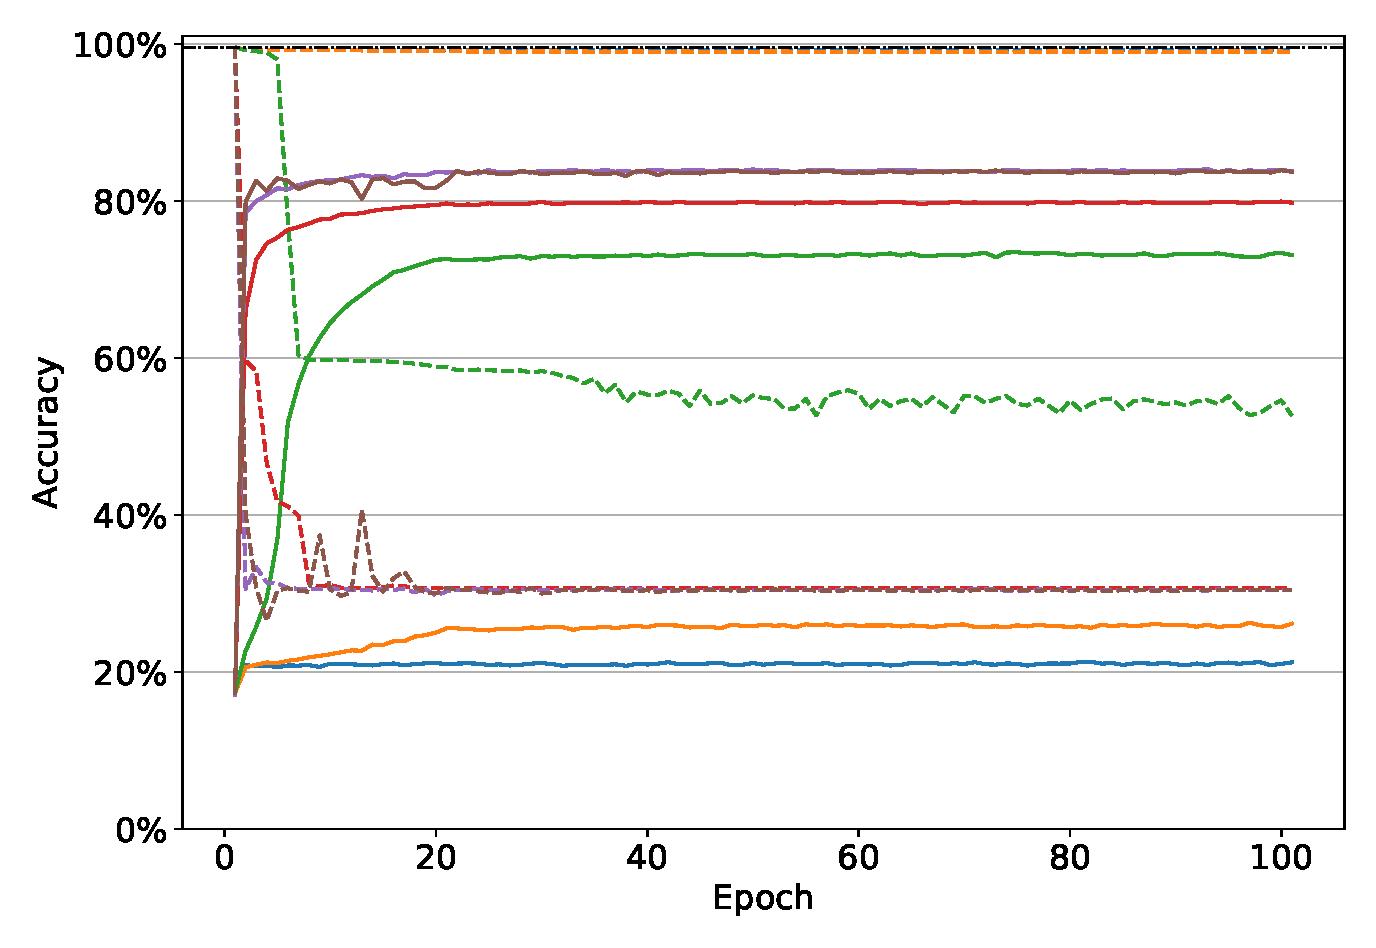
\includegraphics[width=\textwidth]{images/finetuning/finetuning_nonwm_model_thesis_simplenet_mnist_tunealllayers_False.eps}
         \caption{SimpleNet, only last layers}
         \label{fig:finetuning_simplenet_lastlayer}
     \end{subfigure}
     \hfill
     \begin{subfigure}[b]{0.49\textwidth}
         \centering
         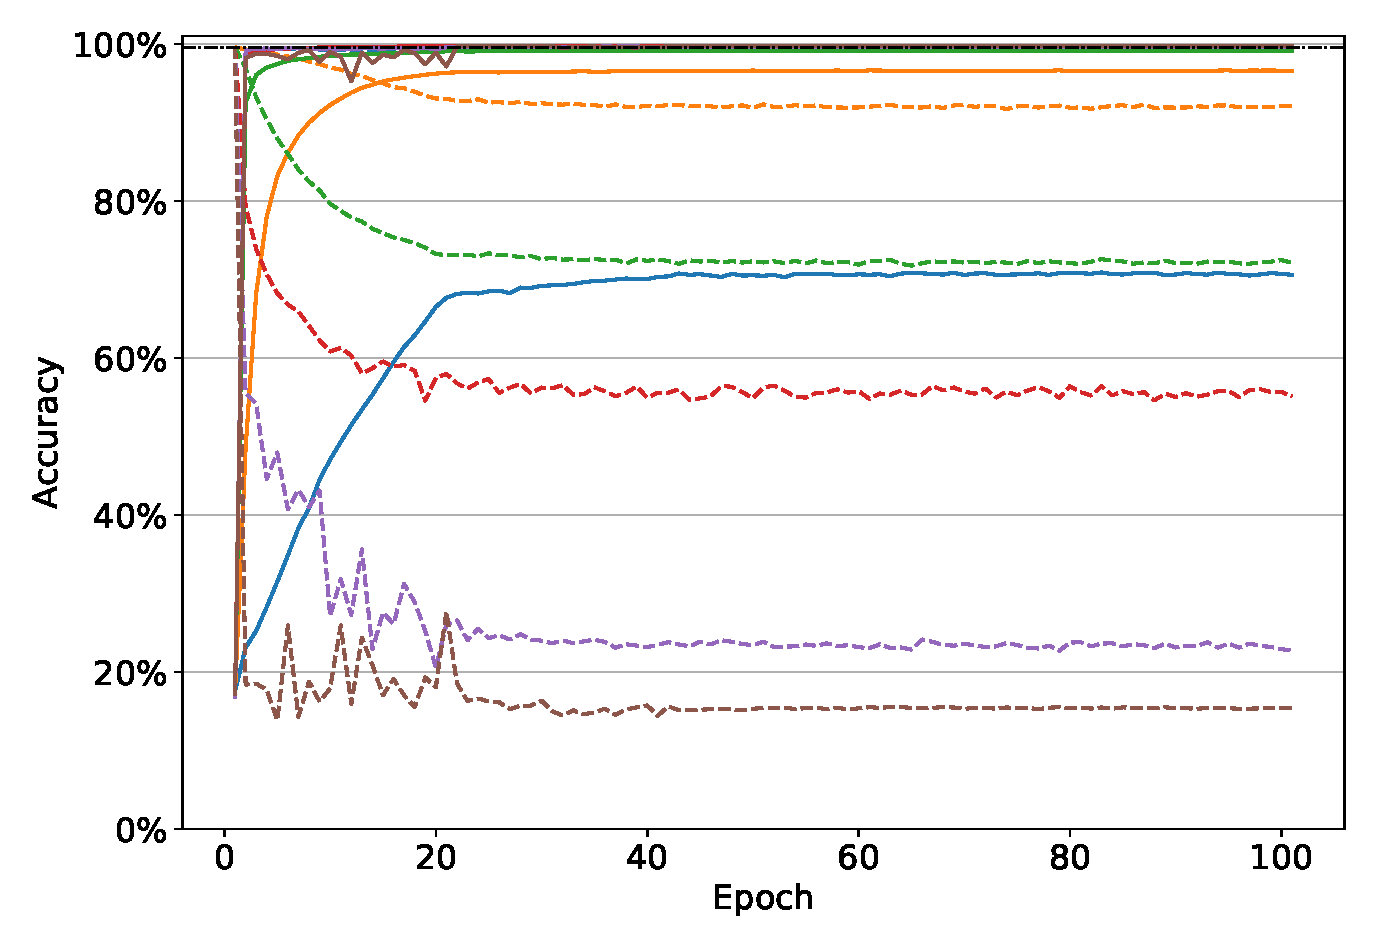
\includegraphics[width=\textwidth]{images/finetuning/finetuning_nonwm_model_thesis_simplenet_mnist_tunealllayers_True.eps}
         \caption{SimpleNet, all layers}
         \label{fig:finetuning_simplenet_alllayers}
     \end{subfigure}
     \hfill
     \begin{subfigure}[b]{\textwidth}
         \centering
         \includegraphics[height=1.1cm]{images/finetuning/legend_finetuning_allvslast_colors.eps}
         \quad
         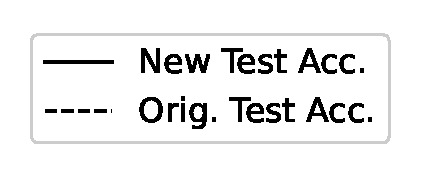
\includegraphics[height=1.1cm]{images/finetuning/legend_finetuning_allvslast_linetypes.eps}

     \end{subfigure}
     \caption{Fine-tuning on non-watermarked SimpleNet. The plot on the left side correspond to fine-tuning only the last layer and the one on the right hand side to fine-tuning all layers. The black dash-dotted line corresponds to the benchmark test accuracy of the non-watermarked model.}
     
     \label{fig:finetuning_all_vs_last_layers}
\end{figure}

First, we compare fine-tuning that trains only the last layer with fine-tuning that trains on all layers. We fine-tune non-watermarked models and conclude that fine-tuning on all layers leads to better results, as we can see, e.g. on SimpleNet, in \cref{fig:finetuning_all_vs_last_layers}. When fine-tuning only the last layer, the model seems to be unable to learn the new data properly. For a small learning rate, e.g. $\alpha=10^{-6}$, when fine-tuning only the last layer, the test accuracy of the new dataset stays at $20\%$ for all iterations, while the test accuracy on the original test set stays at the benchmark. With the same learning rate and fine-tuning all layers, the model is able to learn to predict the new dataset with around $70\%$ accuracy. For a large learning rate, e.g. $\alpha=10^{-2}$, the original test accuracy drops to around $30\%$, regardless of whether fine-tuning only the last layer or all layers. At the same time, when fine-tuning all layers, at least the new test accuracy reaches almost the benchmark score, whereas when fine-tuning only the last layer, the new test accuracy reaches only around $85\%$.

In summary, the original test accuracy behaves similarly in both settings. Even though it is a bit worse when fine-tuning all layers, the new test accuracy reaches better results when fine-tuning all layers. It, of course, depends on the motives of an attacker, but we believe that an attacker would either perform transfer-learning where both the new and the original test accuracy are at an acceptable level ($\alpha=10^{-5}$) or would try to purposefully overfit the new data (e.g. $\alpha=10^{-1}$), in order to let the model "forget" the original data (and watermark). We analyse the influence of different learning rates in the following.

From now on, in the following experiments and also for the evaluation of the robustness of the watermarking methods, we always fine-tune on all layers.

\begin{figure}
\centering
\begin{subfigure}[b]{0.49\textwidth}
    \centering
    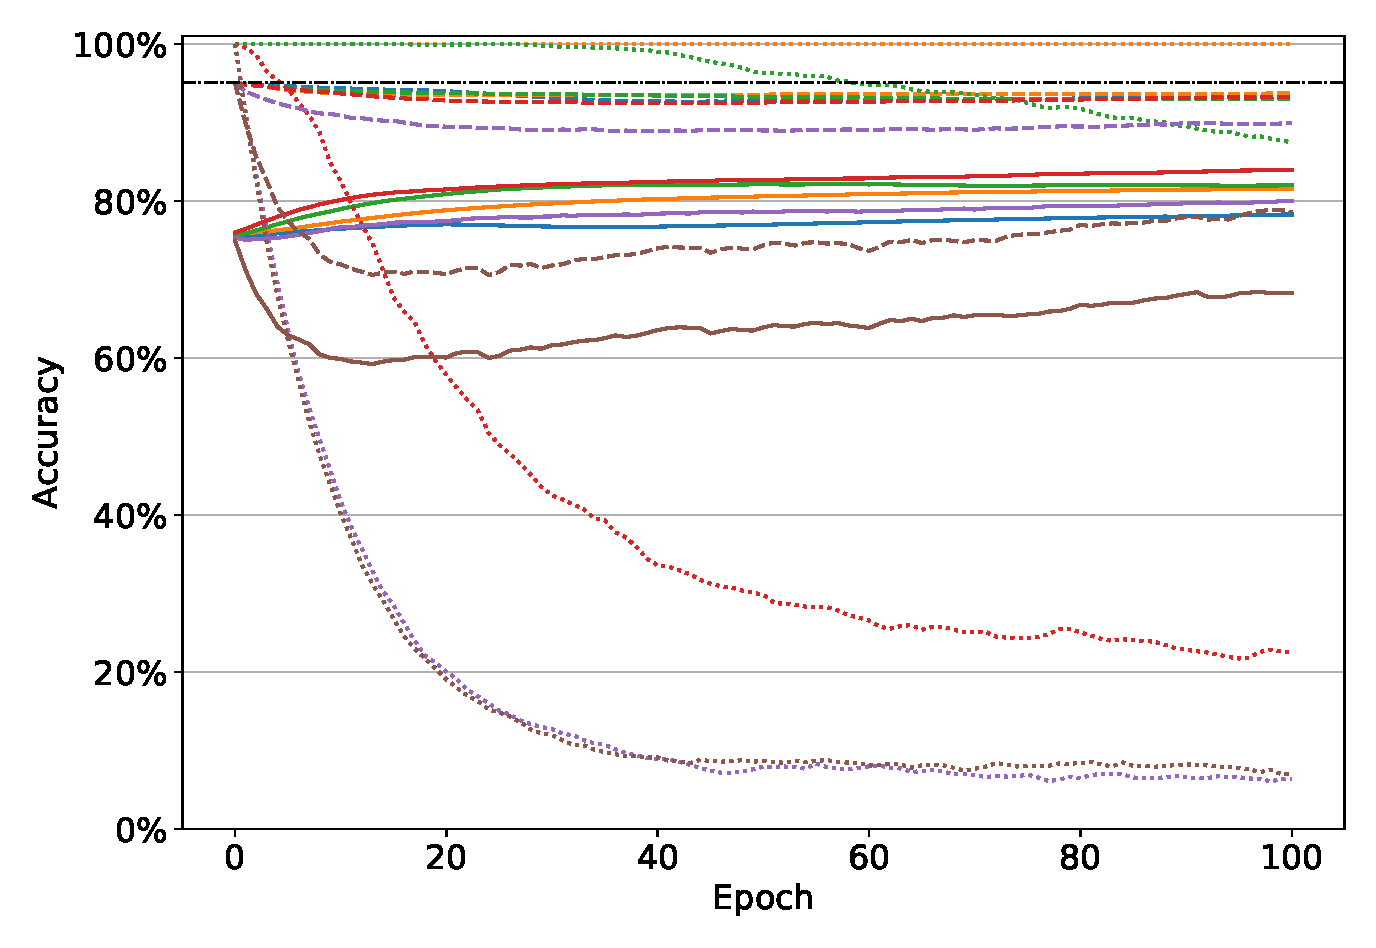
\includegraphics[width=\linewidth]{images/finetuning/finetuning_protecting_content_smoothed_imagenet_0.eps}
    \caption{Fine-Tuning on CINIC-10}
    \label{fig:fine-tuning-cinic10}
\end{subfigure}
\begin{subfigure}[b]{0.49\textwidth}
    \centering
    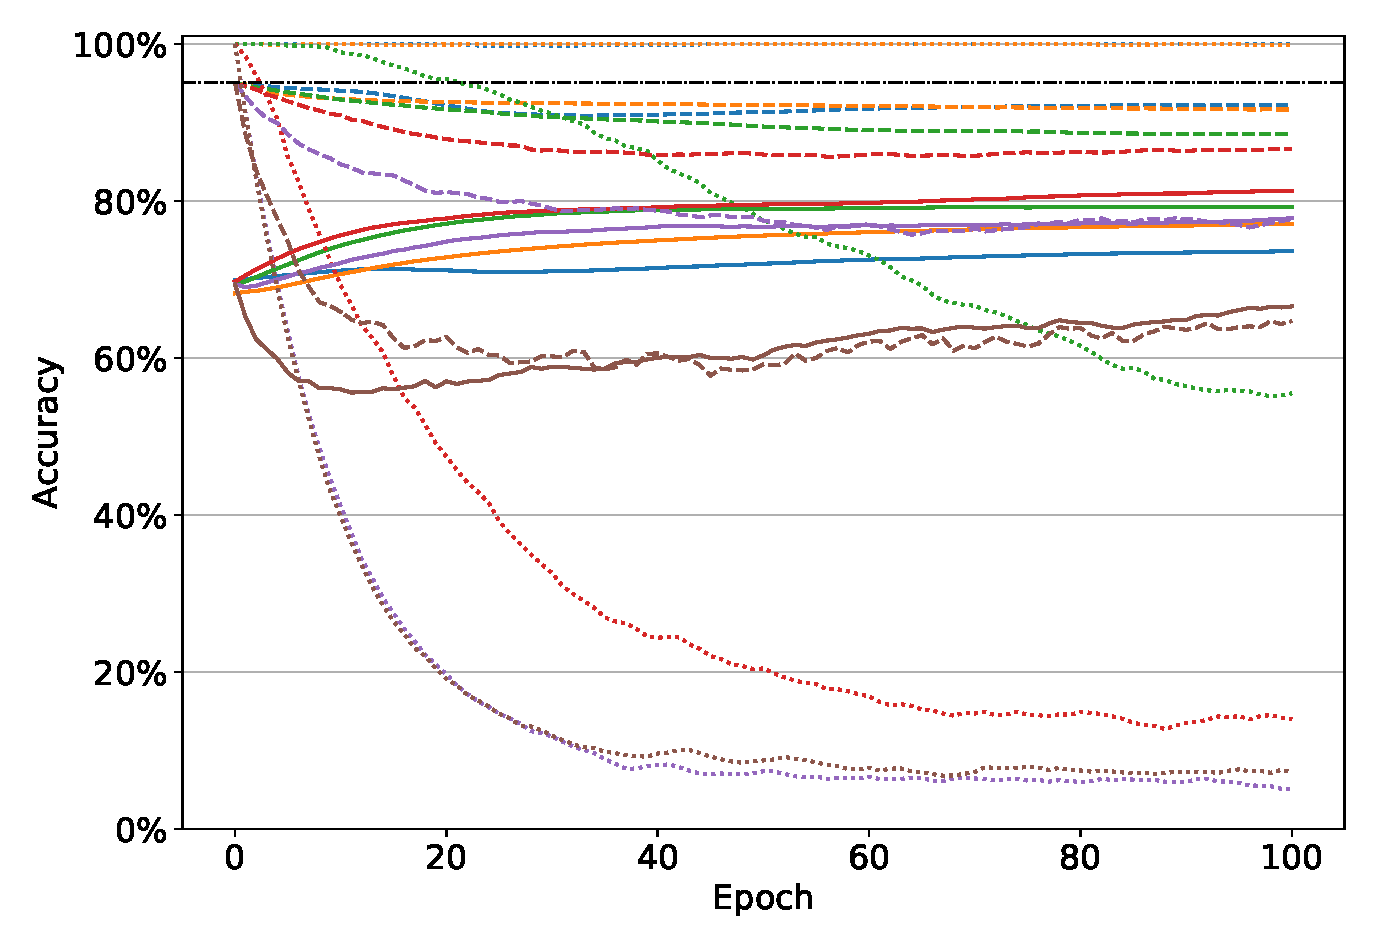
\includegraphics[width=\linewidth]{images/finetuning/finetuning_protecting_content_smoothed_imagenet_1.eps}
    \caption{Fine-Tuning on ImageNet part of CINIC-10}
    \label{fig:fine-tuning-cinic10-imagenet}
\end{subfigure}

\begin{subfigure}[b]{\linewidth}
    \centering
    \includegraphics[height=1.1cm]{images/finetuning/legend_content_finetuning_imagenet_colors.eps}
    \quad
    \includegraphics[height=1.1cm]{images/finetuning/legend_content_finetuning_imagenet_linetypes.eps}
\end{subfigure}

\caption{Fine-Tuning on both, CINIC-10 and only on the ImageNet part of CINIC-10. In both cases, 50,000 images are randomly chosen from the corresponding dataset. The underlying model is a ResNet-18 that was trained with \textit{ProtectingIP-pattern} and 100 trigger images. The black dash-dotted line corresponds to the benchmark test accuracy of the non-watermarked model. For clearity reasons, the lines in the plot are smoothed. The original plots are provided in \cref{fig:fine-tuning-both-cinic10-imagenet-original}.}
\label{fig:fine-tuning-both-cinic10-imagenet}

\end{figure}

Since CINIC-10 is a dataset consisting of 90,000 training images, from which 70,000 are drawn from ImageNet, and we downsample the fine-tuning dataset to 50,000 training images, we could either randomly choose 50,000 training images from CINIC-10 or only from the ImageNet part of CINIC-10. In \cref{fig:fine-tuning-both-cinic10-imagenet} we show the results for fine-tuning on CINIC-10 and on the ImageNet part of CINIC-10 for learning rates from $10^{-6}$ to $10^{-1}$. We conclude that the choice of the dataset does not make much difference on the new test accuracy. However, fine-tuning on the ImageNet part leads to both a quicker original test accuracy and watermark accuracy drop for higher learning rates. In the following, we fine-tune using CINIC-10, as the attacker would also use the most similar dataset for the purpose of transfer-learning. For the purpose of re-training, we see that the watermark accuracy drops below 20\% for large learning rates, anyhow, so the differences in these versions of the data do not have a large effect.

\begin{figure}
     \centering
     \begin{subfigure}[b]{0.49\textwidth}
         \centering
         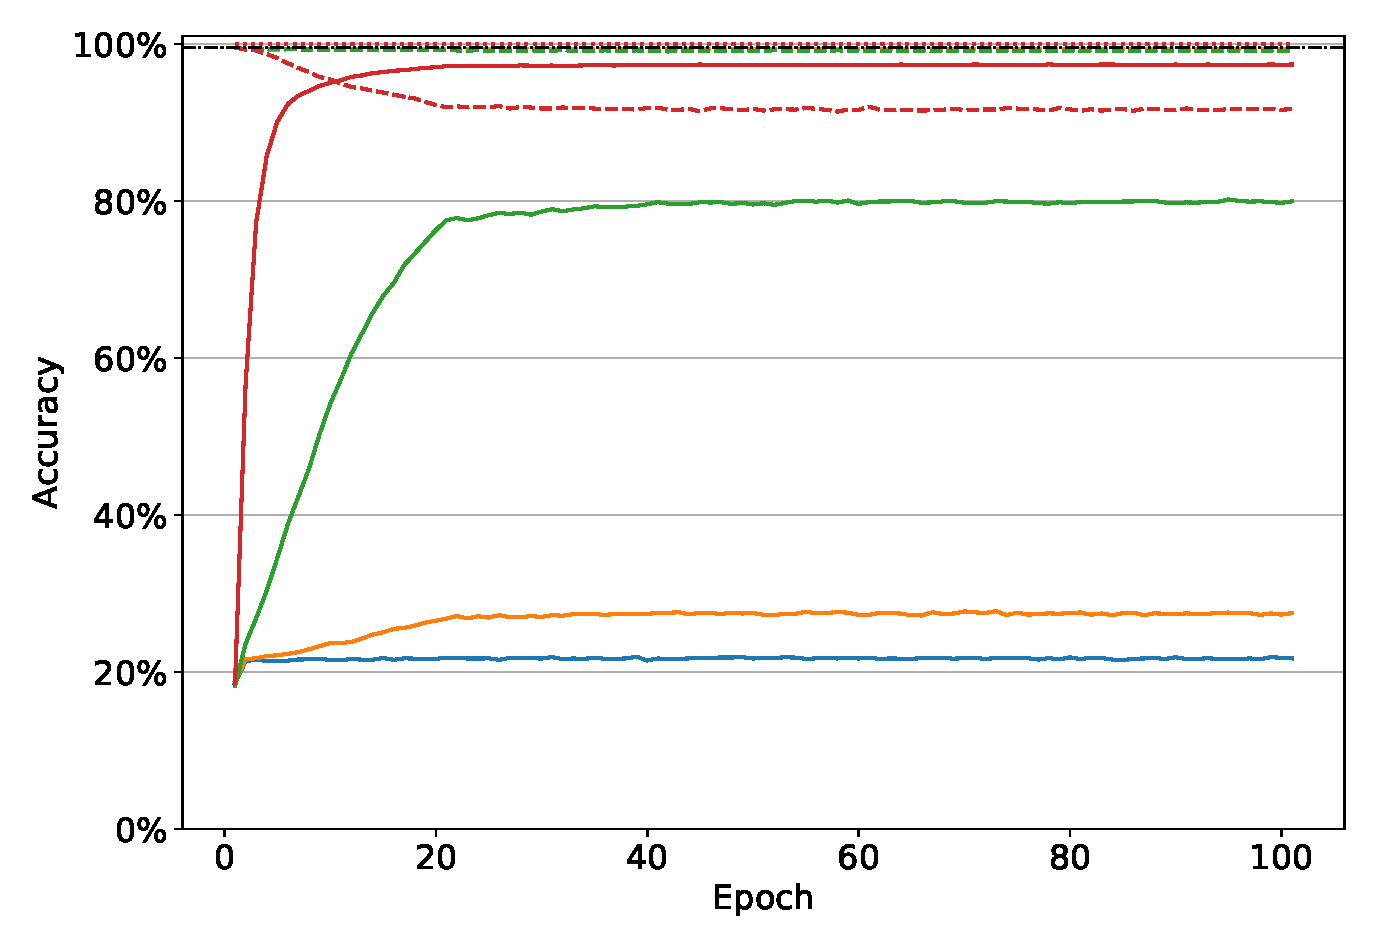
\includegraphics[width=\textwidth]{images/finetuning/finetuning_protecting_content_smalllr_thesis_simplenet_mnist.eps}
         \caption{SimpleNet, small learning rates (MNIST)}
         \label{fig:finetuning_simplenet_smalllr}
     \end{subfigure}
     \hfill
     \begin{subfigure}[b]{0.49\textwidth}
         \centering
         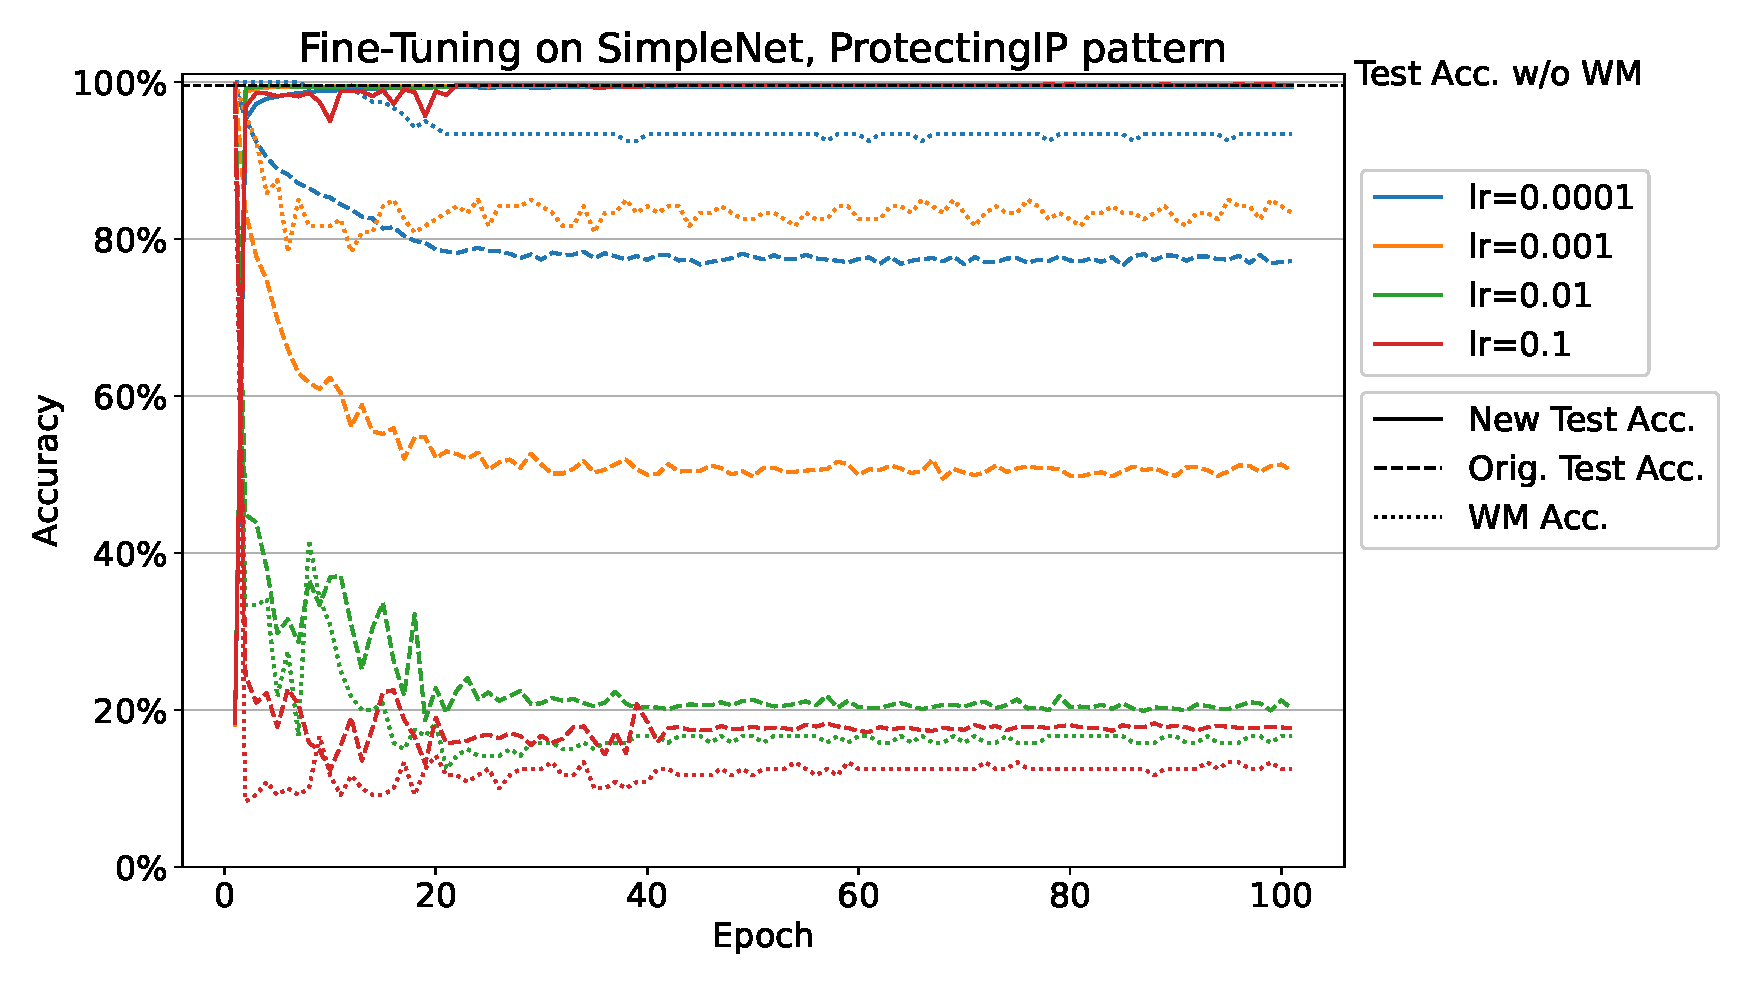
\includegraphics[width=\textwidth]{images/finetuning/finetuning_protecting_content_largelr_thesis_simplenet_mnist.eps}
         \caption{SimpleNet, large learning rates (MNIST)}
         \label{fig:finetuning_simplenet_largelr}
     \end{subfigure}
     \hfill
     \begin{subfigure}[b]{0.49\textwidth}
         \centering
         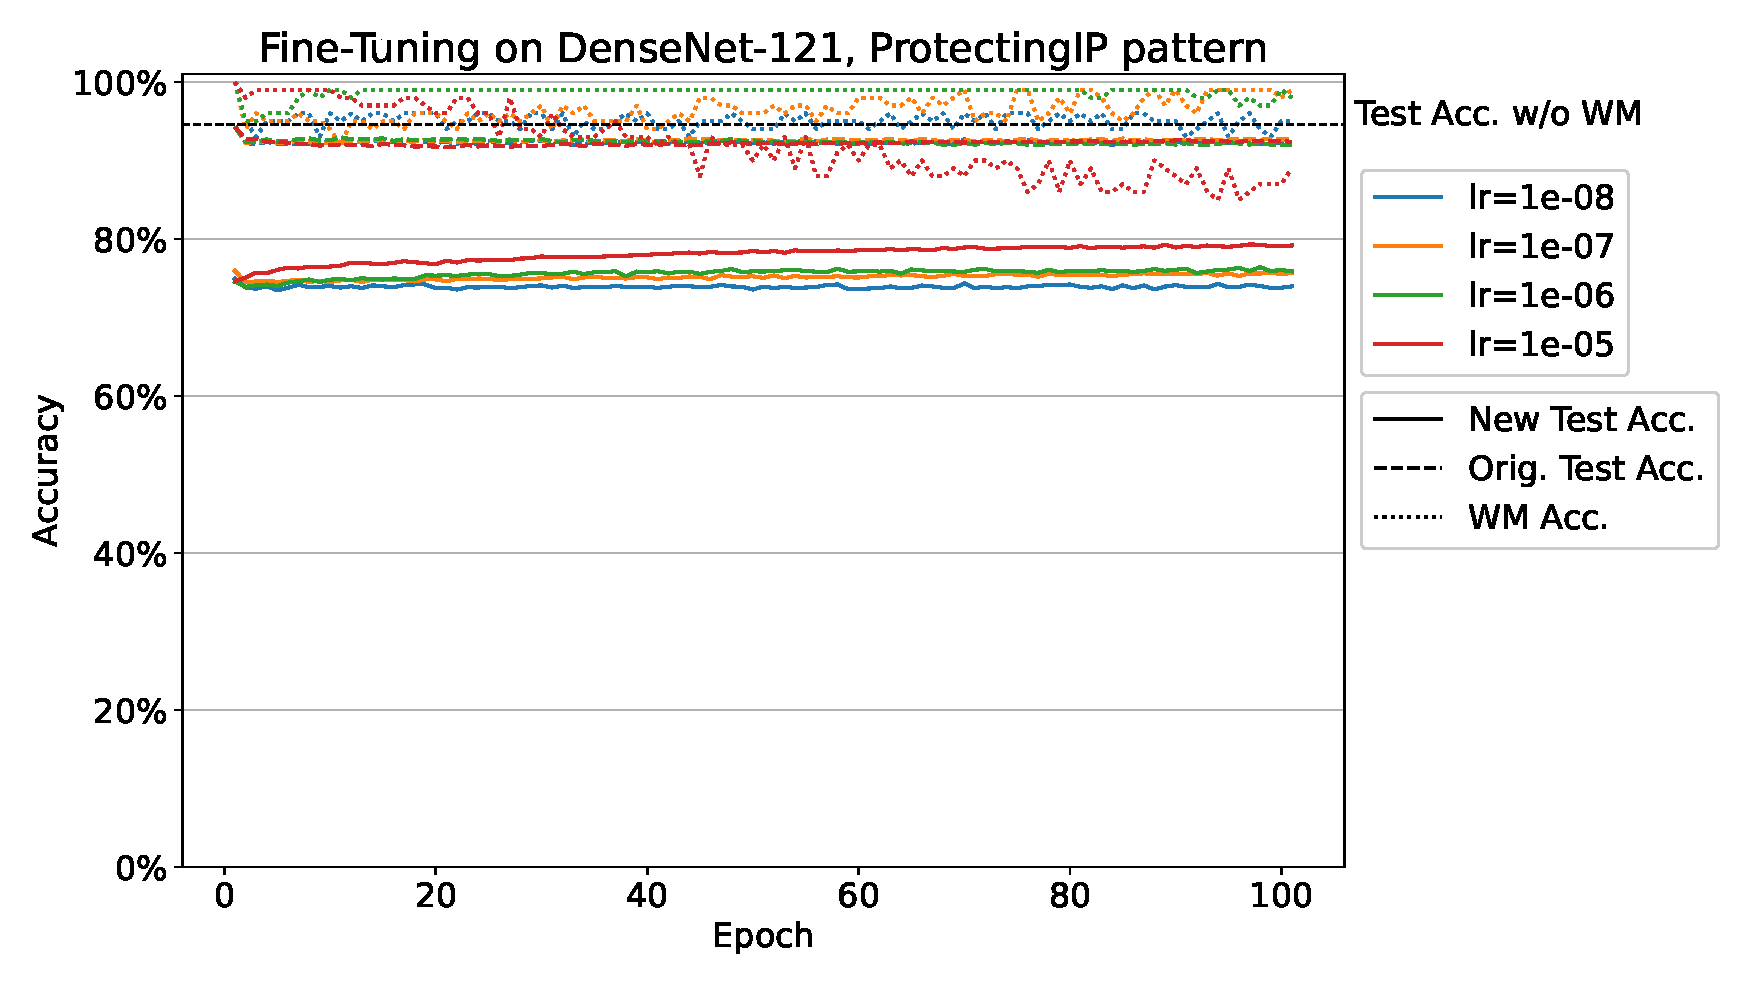
\includegraphics[width=\textwidth]{images/finetuning/finetuning_protecting_content_smalllr_thesis_densenet.eps}
         \caption{DenseNet, small learning rates (CIFAR-10)}
         \label{fig:finetuning_densenet_smalllr}
     \end{subfigure}
     \hfill
     \begin{subfigure}[b]{0.49\textwidth}
         \centering
         \includegraphics[width=\textwidth]{images/finetuning/finetuning_protecting_content_largelr_thesis_densenet.eps}
         \caption{DenseNet, large learning rates (CIFAR-10)}
         \label{fig:finetuning_densenet_largelr}
     \end{subfigure}
     \hfill
     \begin{subfigure}[b]{\textwidth}
         \centering
         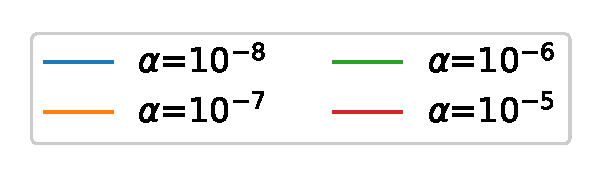
\includegraphics[height=1.1cm]{images/finetuning/legend_content_finetuning_smalllr_colors.eps}
         \quad
         \includegraphics[height=1.3cm]{images/finetuning/legend_content_finetuning_linetypes.eps}
         \quad
         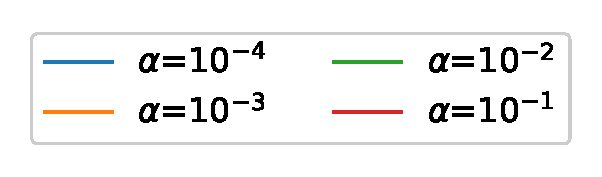
\includegraphics[height=1.1cm]{images/finetuning/legend_content_finetuning_largelr_colors.eps}
     \end{subfigure}
     \caption{Fine-tuning on SimpleNet and DenseNet, watermarked with ProtectingIP-pattern. The plots on the left side correspond to fine-tuning with smaller learning rates and the ones on the right side to fine-tuning with larger learning rates. The black dash-dotted line corresponds to the benchmark test accuracy of the non-watermarked model.}
     
     \label{fig:finetuning_simplenet_and_densenet}
\end{figure}

In another experiment, we test several learning rates in order to see how the choice of learning rate influences (i) the test accuracy on the original dataset, (ii) the test accuracy on the new dataset, and (iii) the watermark accuracy. For selecting a learning rate for attacks on all other watermarking methods, we fine-tune exemplary only on the models that were watermarked with \textit{ProtectingIP-pattern} and with $100$ trigger images. \Cref{fig:finetuning_simplenet_and_densenet} shows the results for DenseNet (on CIFAR-10) and for SimpleNet (on MNIST). Although the behaviour differs much between the two datasets, the behaviour for the models across one dataset is very similar. That is why we focus on DenseNet and SimpleNet as examples here and provide the plots for the other models in \cref{sec:appendix:finetuning-plots}. We can conclude from \cref{fig:finetuning_simplenet_largelr} that fine-tuning on MNIST models with a larger learning rate tends to fit the new data too much and therefore the model "forgets" the original dataset and watermark, i.e. the test accuracy on the original dataset and the watermark accuracy drops already after a few training iterations. This phenomenon is referred to as \textit{catastrophic forgetting} \cite{kirkpatrick_overcoming_2017}. A model fine-tuned with a smaller learning rate, on the other hand, does not tend to overfit and either learns to adapt to the new data with only a little accuracy drop on the original test data ($\alpha=10^{-5}$ in \cref{fig:finetuning_simplenet_smalllr}) or is unable to learn the new data at all ($\alpha=10^{-8}$ in \cref{fig:finetuning_simplenet_smalllr}).

Considering CIFAR-10, shown in \cref{fig:finetuning_densenet_smalllr,fig:finetuning_densenet_largelr}, we do not see this catastrophic forgetting regarding the old training data for any of the learning rates, perhaps because the datasets are too similar. However, we do clearly see that for larger learning rates the watermark accuracy drops, i.e. the model "forgets" the watermarks more quickly.

\subsection{Influence of watermark-specific hyparameters} \label{sec:eval-watermark-spec-param}

In the following subsections, we discuss two methods, namely \textit{FrontierStitching} and \textit{WMEmbeddedSystems}, which we analysed regarding the influence of a method-specific parameter.

\subsubsection{FrontierStitching} \label{sec:eval-param:frontier}

In this section, we analyse how the parameter $\epsilon$ for FGSM influences fidelity and robustness of the watermarking method. We use [0.0001, 0.001, 0.01, 0.1, 0.25, 0.5, 1.0] as $\epsilon$ values. \Cref{fig:frontier_trigger-images} shows examples of trigger images for the different values of $\epsilon$.

\begin{figure}[t]
    \centering
    \hspace*{\fill}
  \subfloat[\label{fig:frontier_eps0.0001} 0.0001]{\includegraphics[width = 0.13 \linewidth]{images/frontier/eps00001.jpg}}
    \hspace*{\fill}
  \subfloat[\label{fig:frontier_eps0.001} 0.001]{\includegraphics[width = 0.13 \linewidth]{images/frontier/eps0001.jpg}}
    \hspace*{\fill}
  \subfloat[\label{fig:frontier_eps0.01} 0.01]{\includegraphics[width = 0.13 \linewidth]{images/frontier/eps001.jpg}}
    \hspace*{\fill}
  \subfloat[\label{fig:frontier_eps0.1} 0.1]{\includegraphics[width = 0.13 \linewidth]{images/frontier/eps01.jpg}}
    \hspace*{\fill}
    \subfloat[\label{fig:frontier_eps0.25} 0.25]{\includegraphics[width = 0.13 \linewidth]{images/frontier/eps025.jpg}}
    \hspace*{\fill}
  \subfloat[\label{fig:frontier_eps0.5} 0.5]{\includegraphics[width = 0.13 \linewidth]{images/frontier/eps05.jpg}}
    \hspace*{\fill}
  \subfloat[\label{fig:frontier_eps1.0} 1.0]{\includegraphics[width = 0.13 \linewidth]{images/frontier/eps10.jpg}}
    \hspace*{\fill}
    \caption{Examples for FrontierStitching trigger images for different values of $\epsilon$, created with FGSM on LeNet-1.}
    \label{fig:frontier_trigger-images}
\end{figure}

When it comes to effectiveness, all models reach $100\%$ watermark accuracy, except of LeNet-5 with $\epsilon=0.25$, which has a watermark accuracy of $68\%$. We see later in \cref{sec:eval-effectiveness} that, at least for $\epsilon=0.25$, the watermark accuracy on LeNet-5 drops with the trigger set size.

%We train on all architectures with a fixed trigger set size of 100  and subsequently perform attacks. 

In the first experiment, we test the influence of the parameter $\epsilon$ on the validation loss difference, e.i. the validation loss of the non-watermarked model subtracted from the validation loss of the watermarked model. We expect that watermarked models trained on trigger images with a larger perturbation lead to a higher performance drop, i.e. the validation loss is higher than for models trained on less perturbed trigger images.

\begin{figure}
    \centering
    %\includegraphics[width = 0.8 \linewidth]{images/frontier/frontier_influence_epsilon_validloss.eps}
    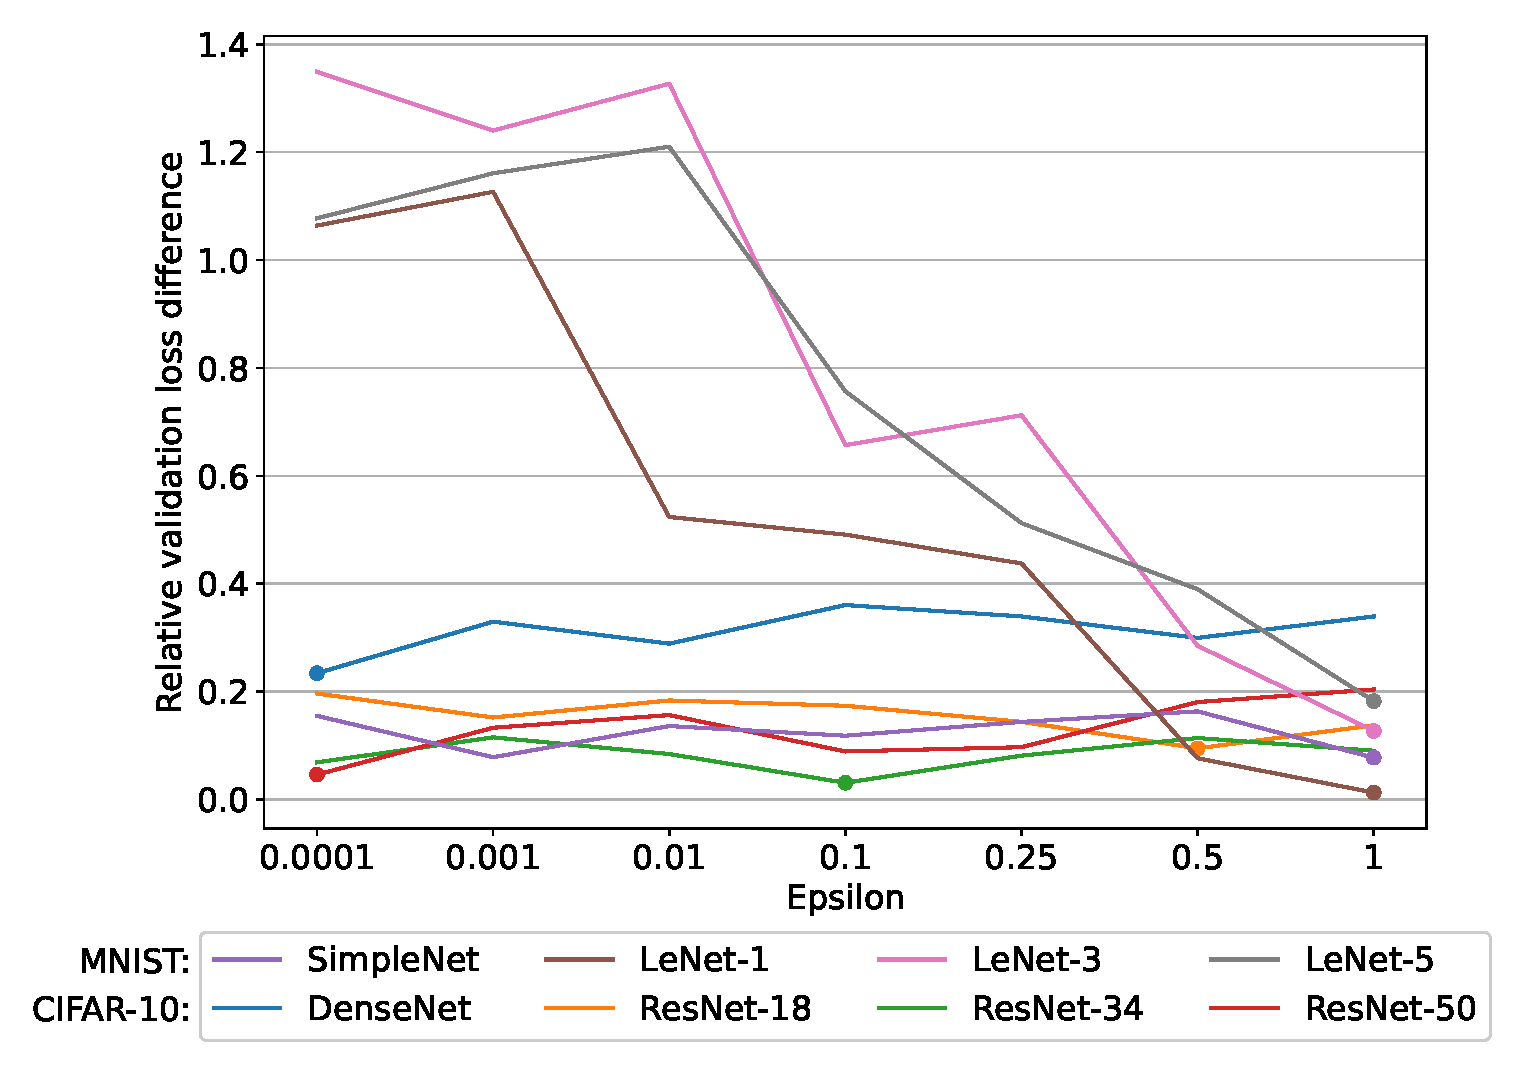
\includegraphics[width = 0.8 \linewidth]{images/frontier/frontier_influence_epsilon_validloss_relative.eps}
    \caption{FrontierStitching with various values for $\epsilon$ (strength of perturbation). The plot shows the relative validation loss difference, i.e. the difference between the validation loss of the watermarked model and the non-watermarked benchmark model divided by the validation loss of the benchmark model. For all values the WM Accuracy is $100\%$. The dots in the plot represent the minimal validation loss difference for the respective architecture.}
    \label{fig:frontier_influence_epsilon}
\end{figure}

The results are summarised in \cref{fig:frontier_influence_epsilon}. We conclude from this experiment that the influence of $\epsilon$ is very much dependent on the architecture. The LeNets tend to perform better with a higher $\epsilon$, as the relative difference in validation loss drops from 1.0-1.4 to 0-0.2. The value of $\epsilon$ does not affect the other models much, as the relative validation loss difference is between in a range of $\pm 0.1$ for all $\epsilon$. For DenseNet and ResNet-50, however, we see a trend that a smaller $\epsilon$ leads to better fidelity.

Since a good watermarking method should not only achieve a good fidelity but also good robustness, we perform pruning and fine-tuning on these models to test robustness. The results for pruned models depend very much on the complexity of the architecture. \cref{fig:frontier_influence_epsilon_pruning} shows the results for LeNet-1 and LeNet-5. The pruning attack affects the smaller architecture much more than the more complex one. Even with a small pruning rate of 20\%, both the test and watermark accuracy of LeNet-1 start to drop. Compared to this, a LeNet-5 does not change in performance until 70\% of the weights are pruned. This could indicate that LeNet-5 has spare capacity and is more complex than needed for the task.

%In order to find the most suitable parameter $\epsilon$, we introduce the following ranking system: we tested on six different values for $\epsilon$ (c.f. \cref{fig:frontier_trigger-images}), therefore we give points from 1 to 6 depending on the performance in the categories \textit{fidelity}, \textit{robustness against pruning} and \textit{robustness against fine-tuning}. Six points mean that the model performs best in the corresponding category and one point means it performs worst compared to the other models with a different $\epsilon$. For the category \textit{fidelity}, we give the model with the least validation loss error six points and the model with the highest validation loss error one point. Validation loss error means the difference between the validation loss of the non-watermarked model and the watermarked model. To give an example, we can see from \cref{fig:frontier_influence_epsilon} that the ranking for DenseNet-121 is the following:

%\begin{itemize}
%    \item 6 points for $\epsilon$=0.0001.
%    \item 5 points for $\epsilon$=0.01.
%    \item 4 points for $\epsilon$=0.5.
%    \item 3 points for $\epsilon$=0.001.
%    \item 2 points for $\epsilon$=1.
%    \item 1 point for $\epsilon$=0.1.
%\end{itemize}


\begin{figure}
    \centering
    \begin{subfigure}[b]{0.49\linewidth}
    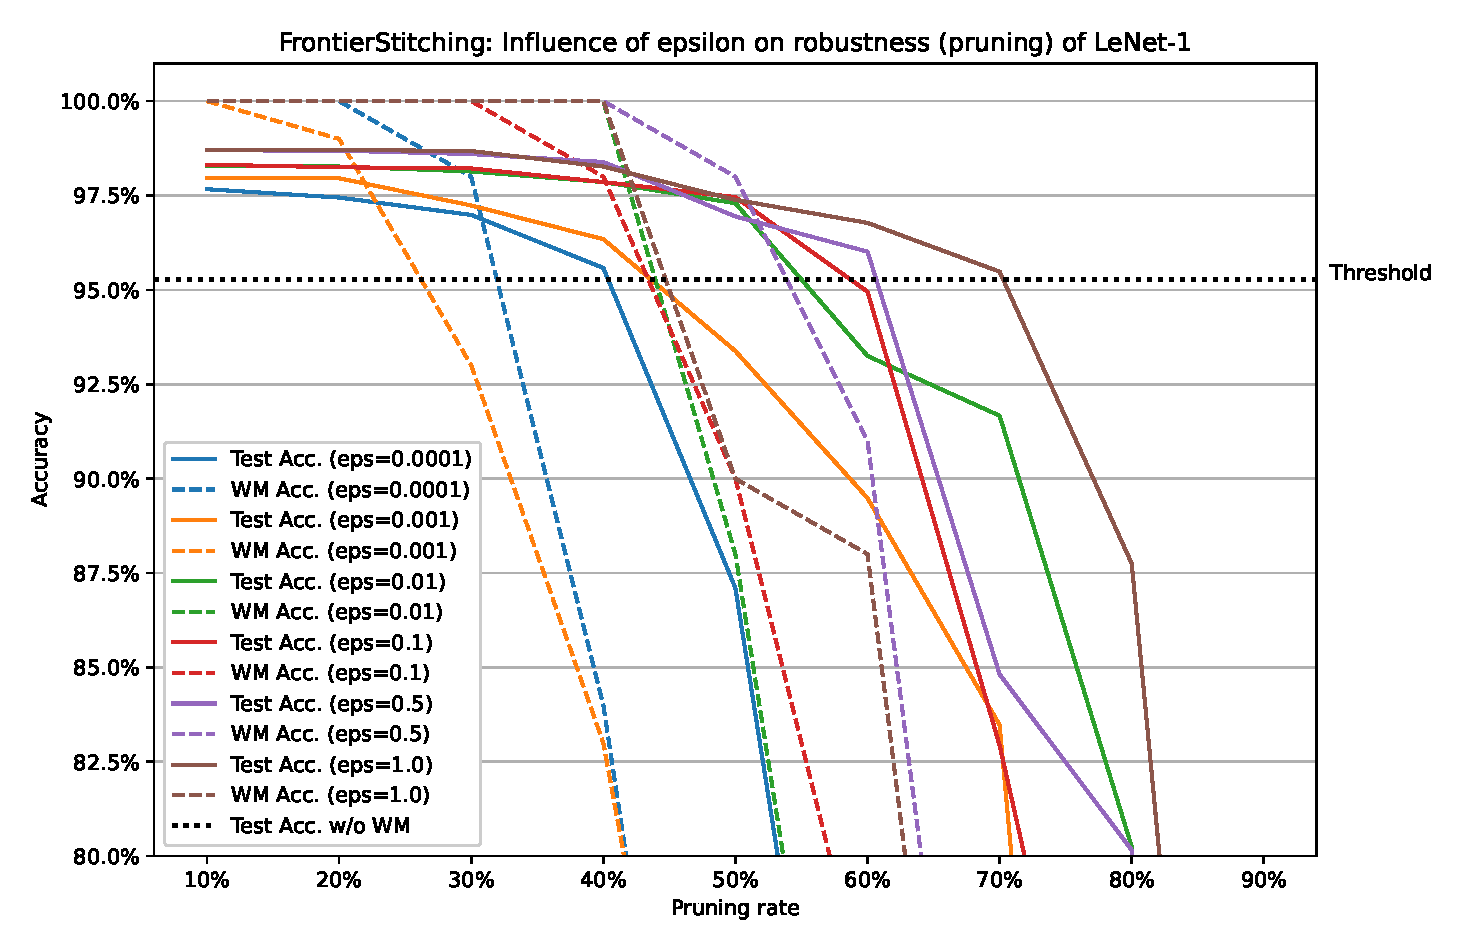
\includegraphics[width = \linewidth]{images/frontier/frontier_influence_epsilon_pruning_lenet1.eps}
    \caption{LeNet-1}
    \label{fig:frontier_influence_epsilon_pruning-a}
    \end{subfigure}
    \begin{subfigure}[b]{0.49\linewidth}
    \includegraphics[width = \linewidth]{images/frontier/frontier_influence_epsilon_pruning_lenet5.eps}
    \caption{LeNet-5}
    \label{fig:frontier_influence_epsilon_pruning-b}
    \end{subfigure}
    \begin{subfigure}[b]{\linewidth}
    \centering
    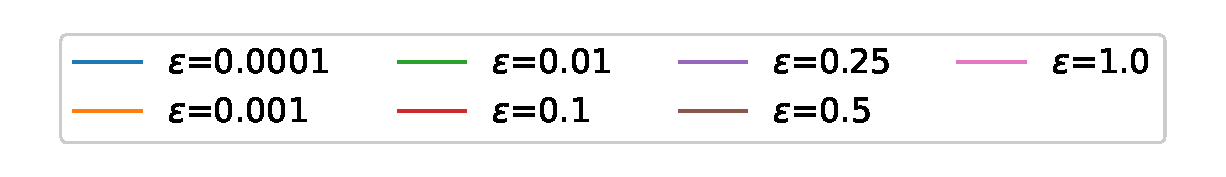
\includegraphics[height=1cm]{images/frontier/legend_frontier_pruning_perarch_colors.eps}
    \quad
    \includegraphics[height=1cm]{images/frontier/legend_frontier_pruning_perarch_linetypes.eps}
    \end{subfigure}
    
    \caption{Model accuracy after pruning attacks with pruning rates from 10\% to 90\%. The black dotted line indicates the threshold for the maximal plausible pruning attack.}
    \label{fig:frontier_influence_epsilon_pruning}
\end{figure}

As already discussed in \cref{sec:implementation:pruning}, we consider a pruning attack as plausible when the test accuracy drops $3.5\%$ at maximum. In \cref{fig:frontier_influence_epsilon_pruning} this threshold is marked with a black dotted line. For instance, we see that the maximal plausible pruning rate for LeNet-5 in \cref{fig:frontier_influence_epsilon_pruning-b} is 90\% for all values of $\epsilon$, whereas for LeNet-1 in \cref{fig:frontier_influence_epsilon_pruning-a} it very much depends on the parameter $\epsilon$. The maximal plausible pruning rate for LeNet-1, e.g., for the values $0.0001$ and $0.001$ is $40\%$, for $0.5$ it is $60\%$ and $1.0$ it is $70\%$.
%We get a ranking for the models for this category by comparing the watermark accuracies at the maximal pausible pruning rate. As we can see in \cref{fig:frontier_influence_epsilon_pruning-b}, the maximal plausible pruning rate for LeNet-5 is $90\%$ for all $\epsilon$. The ranking for LeNet-5 is then the following:

%\begin{itemize}
%    \item 6 points for $\epsilon$=0.5 (WM Acc. $70\%$ at $90\%$ pruning rate)
%    \item 5 points for $\epsilon$=1.0 (WM Acc. $59\%$ at $90\%$ pruning rate)
%    \item 4 points for $\epsilon$=0.1 (WM Acc. $58\%$ at $90\%$ pruning rate)
%    \item 2.5 points for both $\epsilon$=0.0001 and $\epsilon$=0.01 (WM Acc. $49\%$ at $90\%$ pruning rate)
%    \item 1 point for $\epsilon$=0.001 (WM Acc. $43\%$ at $90\%$ pruning rate)
%\end{itemize}

As the third and last experiment, we perform a fine-tuning attack on the models. First, we assume that an attacker would perform a fine-tuning attack with the purpose of removing the watermark and would therefore choose a relatively high learning rate (cf. \cref{sec:finetuning-experiments}, where we tested several learning rates and analysed the behaviour of the attacked model). We choose $0.01$ as the learning rate for both MNIST and CIFAR-10, based on the experiments in \cref{sec:finetuning-experiments}. Unfortunately, for all models, the watermark accuracy after the fine-tuning attack with a large learning rate is below $20\%$. Second, we perform a fine-tuning attack with a relatively low learning rate (cf. \cref{sec:finetuning-experiments}). We choose $10^{-5}$ for MNIST and $10^{-4}$ for CIFAR-10, based on the experiments in \cref{sec:finetuning-experiments}. After fine-tuning with this small learning rate, the watermark accuracy stays above $50\%$ for most of the models. We summarised the results in \cref{tab:frontier-finetuning}. %We rank the models according to their watermark accuracy after the fine-tuning attack with a small learning rate, according to the same scheme as before.

\begin{table}
\small
\centering
\caption{Watermark accuracies after fine-tuning attack on models trained with FrontierStitching.}
%\rowcolors{2}{white}{gray!15}
\begin{tabular}{|l|l|r|r|l|l|r|r|}
\hline
\multicolumn{4}{|c|}{\textbf{CIFAR-10}} & \multicolumn{4}{c|}{\textbf{MNIST}}     \\ \hline
Arch.     & $\epsilon$    & lr=$10^{-2}$ & lr=$10^{-4}$ & Arch.     & $\epsilon$    & lr=$10^{-2}$ & lr=$10^{-5}$ \\ \hline
DenseNet  & 0.0001 & 6\%     & 65\%     & SimpleNet & 0.0001 & 12\%    & 100\%    \\ \hline
          & 0.001  & 8\%     & 68\%     &           & 0.001  & 12\%    & 97\%     \\ \hline
          & 0.01   & 9\%     & 74\%     &           & 0.01   & 9\%     & 100\%    \\ \hline
          & 0.1    & 10\%    & 68\%     &           & 0.1    & 12\%    & 94\%     \\ \hline
          & 0.25   & 11\%    & 75\%     &           & 0.25   & 9\%     & 92\%     \\ \hline
          & 0.5    & 15\%    & 53\%     &           & 0.5    & 10\%    & 96\%     \\ \hline
          & 1      & 13\%    & 24\%     &           & 1      & 12\%    & 92\%     \\ \hline
ResNet-18 & 0.0001 & 11\%    & 76\%     & LeNet-1   & 0.0001 & 12\%    & 46\%     \\ \hline
          & 0.001  & 17\%    & 82\%     &           & 0.001  & 12\%    & 54\%     \\ \hline
          & 0.01   & 11\%    & 86\%     &           & 0.01   & 10\%    & 43\%     \\ \hline
          & 0.1    & 13\%    & 86\%     &           & 0.1    & 10\%    & 59\%     \\ \hline
          & 0.25   & 4\%     & 94\%     &           & 0.25   & 11\%    & 57\%     \\ \hline
          & 0.5    & 9\%     & 67\%     &           & 0.5    & 11\%    & 74\%     \\ \hline
          & 1      & 9\%     & 53\%     &           & 1      & 10\%    & 63\%     \\ \hline
ResNet-34 & 0.0001 & 15\%    & 60\%     & LeNet-3   & 0.0001 & 8\%     & 51\%     \\ \hline
          & 0.001  & 14\%    & 69\%     &           & 0.001  & 7\%     & 66\%     \\ \hline
          & 0.01   & 8\%     & 78\%     &           & 0.01   & 6\%     & 53\%     \\ \hline
          & 0.1    & 13\%    & 57\%     &           & 0.1    & 11\%    & 74\%     \\ \hline
          & 0.25   & 12\%    & 71\%     &           & 0.25   & 9\%     & 48\%     \\ \hline
          & 0.5    & 12\%    & 49\%     &           & 0.5    & 11\%    & 37\%     \\ \hline
          & 1      & 13\%    & 48\%     &           & 1      & 9\%     & 51\%     \\ \hline
ResNet-50 & 0.0001 & 8\%     & 93\%     & LeNet-5   & 0.0001 & 7\%     & 45\%     \\ \hline
          & 0.001  & 8\%     & 97\%     &           & 0.001  & 9\%     & 40\%     \\ \hline
          & 0.01   & 9\%     & 99\%     &           & 0.01   & 6\%     & 65\%     \\ \hline
          & 0.1    & 15\%    & 100\%    &           & 0.1    & 7\%     & 55\%     \\ \hline
          & 0.25   & 15\%    & 66\%     &           & 0.25   & 8\%     & 21\%     \\ \hline
          & 0.5    & 8\%     & 99\%     &           & 0.5    & 5\%     & 58\%     \\ \hline
          & 1      & 14\%    & 65\%     &           & 1      & 6\%     & 57\%     \\ \hline
\end{tabular}

\label{tab:frontier-finetuning}
\end{table}



%For evaluating the other watermarking methods, we will only consider fine-tuning with a small learning rate for the ranking.

%Similar, to the evaluation after the pruning attack, we rate the models depending on the watermark accuracy after the performed fine-tuning attack. The results for SimpleNet are shown in \cref{fig:frontier_influence_epsilon_fine-tuning}. \red{COMMENTS}

%After assigning the points in each category to each model, we sum up the points across the categories and get an overall ranking of the performance depending on $\epsilon$ for each architecture, which is summarised in \cref{tab:frontier_ranking}.

%\begin{table}
\small
    \centering
    %\rowcolors{2}{white}{gray!15}
    \caption{Results for ranking system for FrontierStitching. The bold numbers are the highest number for each architecture and indicate the winning $\epsilon$.}
    \begin{tabular}{|l|l|l|l|l|l|l|}
        \hline
        \textbf{Arch.} & $\epsilon=0.0001$ & $\epsilon=0.001$ & $\epsilon=0.01$  & $\epsilon=0.1$ & $\epsilon=0.5$ & $\epsilon=1.0$ \\ \hline
        DenseNet  & 14   & 12.5 & \textbf{16}   & 10.5 & 11   & 4    \\ \hline
        ResNet-18 & 7.5  & 11.5 & 11   & \textbf{12}   & 11.5 & 9.5  \\ \hline
        ResNet-34 & 12.5 & 9.5  & \textbf{13.5} & 12.5 & 7.5  & 7.5  \\ \hline
        ResNet-50 & \red{TODO}     &  \red{TODO}    &  \red{TODO}    &   \red{TODO}   &  \red{TODO}    &  \red{TODO}    \\ \hline
        SimpleNet & 11   & \textbf{12.5} & 12   & 9.5  & 7.5  & 10.5 \\ \hline
        LeNet-1   & 7    & 7    & 10   & 10   & \textbf{17}   & 12   \\ \hline
        LeNet-3   & 5.5  & 12   & 7    & \textbf{16}   & 11   & 11.5 \\ \hline
        LeNet-5   & 7.5  & 4    & 9.5  & 11   & \textbf{16}   & 15   \\ \hline
    \end{tabular}
    \label{tab:frontier_ranking}
\end{table}



\subsubsection{WMEmbeddedSystems}
\label{sec:eval-param:embedded}

Since the authors of the paper do not mention which specific value $\lambda$ (the magnitude or strength of the pattern on the trigger images) they used, we have to find the optimal value for $\lambda$. We want to find a specific value for $\lambda$ for each dataset, but not for each architecture, since the watermark generation does not depend on the model itself and should therefore be created in the same manner for all architectures trained on the same dataset. We average the points for each $\lambda$, grouped by the dataset. The ranking system is presented in \cref{tab:embedded_ranking}. The winning magnitude $\lambda$ for CIFAR-10 is $0.1$ and for MNIST $1.0$.

%We choose the value for $\lambda$ according to the performance on SimpleNet for the models for MNIST and according to the performance on ResNet-34 for the models for CIFAR-10. We recall that in \cref{sec:frontier} we evaluated the parameter $\epsilon$ on every architecture because the perturbation-based watermarking method is very much dependent on the specific architecture.

%Interessante Beobachtung: lenet1 trainiert mit ADAM optimizer -> sehr schlechte Ergebnisse, probiert mit SGD -> bessere und vergleichbar gute Ergebniss! -> Trainiere wm embedded systems mit SGD

\begin{table}
\small
    \centering
    %\rowcolors{2}{white}{gray!15}
    \caption{Results for ranking system for WMEmbeddedSystems. The points are averaged for each dataset and the bold numbers indicate the highest average for each dataset and therefore the winning $\epsilon$.}
\begin{tabular}{|c|l|l|l|l|}
\hline
 & \textbf{Arch.} & $\lambda = 0.1$            & $\lambda = 0.5$   & $\lambda = 1.0$           \\ \hline
{\multirow{5}{*}{\rotatebox[origin=c]{90}{CIFAR-10}}} & DenseNet       & \textbf{6}              & \textbf{6}     & \textbf{6}             \\ \cline{2-5}
& ResNet-18      & \textbf{7}              & 4     & \textbf{7}             \\ \cline{2-5}
& ResNet-34      & \textbf{8}              & 4.5   & 5.5           \\ \cline{2-5}
& ResNet-50      & \textbf{8.5}            & 4.5   & 5             \\ \cline{2-5}
\cline{2-5}
& \textbf{Average}        & \textbf{7.375} & 4.75  & 5.875         \\ \hline
\hline
{\multirow{5}{*}{\rotatebox[origin=c]{90}{MNIST}}} & SimpleNet      & 4              & 6     & \textbf{8}             \\ \cline{2-5}
& LeNet-1        & 3.5            & \textbf{4.5}   & 4             \\ \cline{2-5}
& LeNet-3        & \textbf{7}              & 6     & 5             \\ \cline{2-5}
& LeNet-4        & \textbf{7}              & 5     & 6             \\ \cline{2-5}
\cline{2-5}
& \textbf{Average}        & 5.375          & 5.375 & \textbf{5.75} \\ \hline

\end{tabular}
    \label{tab:embedded_ranking}
\end{table}


%\subsubsection{Blackmarks}
%\label{sec:eval-param:blackmarks}

%\begin{table}
\small
    \centering
    %\rowcolors{2}{white}{gray!15}
    \caption{Results for ranking system for Blackmarks. The bold numbers are the highest number for each architecture and indicate the winning $\epsilon$.}
    \begin{tabular}{|l|l|l|l|l|l|l|}
        \hline
        \textbf{Arch.} & $\epsilon=0.001$ & $\epsilon=0.01$  & $\epsilon=0.1$ & $\epsilon=0.5$ & $\epsilon=1.0$ \\ \hline
        DenseNet  & 9.5         & 9.5          & \textbf{12}  & 11          & 3             \\ \hline
        ResNet-18 & 10 & \textbf{10}  & 8            & 8           & 9             \\ \hline
        ResNet-34 & \textbf{12} & 12  & 7            & 7           & 7             \\ \hline
        SimpleNet & 7           & 9.5          & 9.5          & 6.5         & \textbf{12.5} \\ \hline
        LeNet-1   & 7           & 6            & 9            & 11          & \textbf{12}   \\ \hline
        LeNet-3   & 9           & 10           & \textbf{11}  & 8.5         & 6.5           \\ \hline
        LeNet-5   & 7.5         & 7.5          & 7            & \textbf{13} & 10            \\ \hline
    \end{tabular}
    \label{tab:blackmarks_ranking}
\end{table}

%We follow the ranking system as explained in \cref{sec:studysettings:watermark-spec} and present the results in \cref{tab:blackmarks_ranking}. Note that for ResNet-18 and ResNet-34 the ranking system provides two winning values for $\epsilon$. For those, we choose the one with better robustness against fine-tuning, since the difference in fidelity is negligible. For instance, the exact values for ResNet-18 and ResNet-34 for validation loss and test accuracy are shown in \cref{tab:blackmarks-ranking-fidelity-resnet18/34}.

%\begin{table}
\small
    \centering
    %\rowcolors{2}{white}{gray!15}
    \caption{Results for ranking system for Blackmarks. The bold numbers are the highest number for each architecture and indicate the winning $\epsilon$.}
    \label{tab:blackmarks-ranking-fidelity-resnet18/34}
    \begin{tabular}{|l|l|l|}
        \hline
        \textbf{Model} & Valid. loss & Test Acc. \\
        \hline
        ResNet-18, $\epsilon=0.001$ &  0.056959   &  94.201\%     \\
        \hline 
        ResNet-18, $\epsilon=0.01$  &  0.064496   &   94.201\%    \\
        \hline 
        ResNet-34, $\epsilon=0.001$ & 0.035647    &   94.611\%   \\
        \hline 
        ResNet-34, $\epsilon=0.01$  & 0.032089    &  94.641\%     \\
        \hline 
    \end{tabular}
\end{table}
\clearpage

\subsection{Comparing to State of the Art} \label{sec:compare-results}

In this section, we compare our results to the results in the literature. Note that several results are not fully comparable because of the different study settings, e.g. a custom architecture or unknown trigger set size. Some of the methods focus on a special attack and therefore do not present data that is relevant to our work. \textit{PiracyResistant} \cite{li_piracy_2020} focuses on piracy resistance and \textit{ExponentialWeighting} \cite{namba_robust_2019} on their own crafted attack.
Not knowing all hyper-parameters used in literature further hinders achieving the exact results from related work.

\subsubsection{WeaknessIntoStrength} \label{sec:compare-results:weakness}

Adi et al. \cite{adi_turning_2018} train a ResNet-18 on CIFAR-10, CIFAR-100 and ImageNet with 100 trigger images. We compare the author's results for ResNet-18 on CIFAR-10 with our results. For fidelity, the authors presented results on the test and watermark accuracy after watermark embedding \textit{fromscratch} and \textit{pretrained}. We extract the same information from our models and summarise both, our and the author's results, in \cref{tab:results-fidelity:weakness:compared}. While the authors have a marginal increase, we have a marginal drop in accuracy in the watermarked model compared to the non-watermarked one, but both differences seem negligible. We can also confirm that embedding \textit{fromscratch} leads to better results than embedding the watermark in a \textit{pretrained} model.

%\begin{figure}
%    \centering
%    \includegraphics[width=0.5\linewidth]{images/weakness/weakness_paper_fidelity.png}
%    \caption{Results on fidelity from Adi et al. \cite{adi_turning_2018}.}
%    \label{fig:results-fidelity:weakness}
%\end{figure}

\begin{table}
\centering
\caption{Fidelity results from Adi et al. (\cite{adi_turning_2018}, Table 1), and our experiments.}
\label{tab:results-fidelity:weakness:compared}
\begin{tabular}{|l|l|l||l|l|}
\hline
& \multicolumn{2}{c|}{Adi et al.'s results} & \multicolumn{2}{c|}{Our results}  \\ \hline
Model          & Test Acc.    & WM Acc.        & Test Acc. & WM Acc. \\ \hline
No WM          & 93.42        & 7.0               & 95.122    & -       \\ \hline
Fromscratch    & 93.81        & 100.0       & 94.94     & 100.0   \\ \hline
Pretrained     & 93.65        & 100.0        & 94.61     & 100.0   \\ \hline
\end{tabular}
\end{table}

\begin{figure}
    \centering
    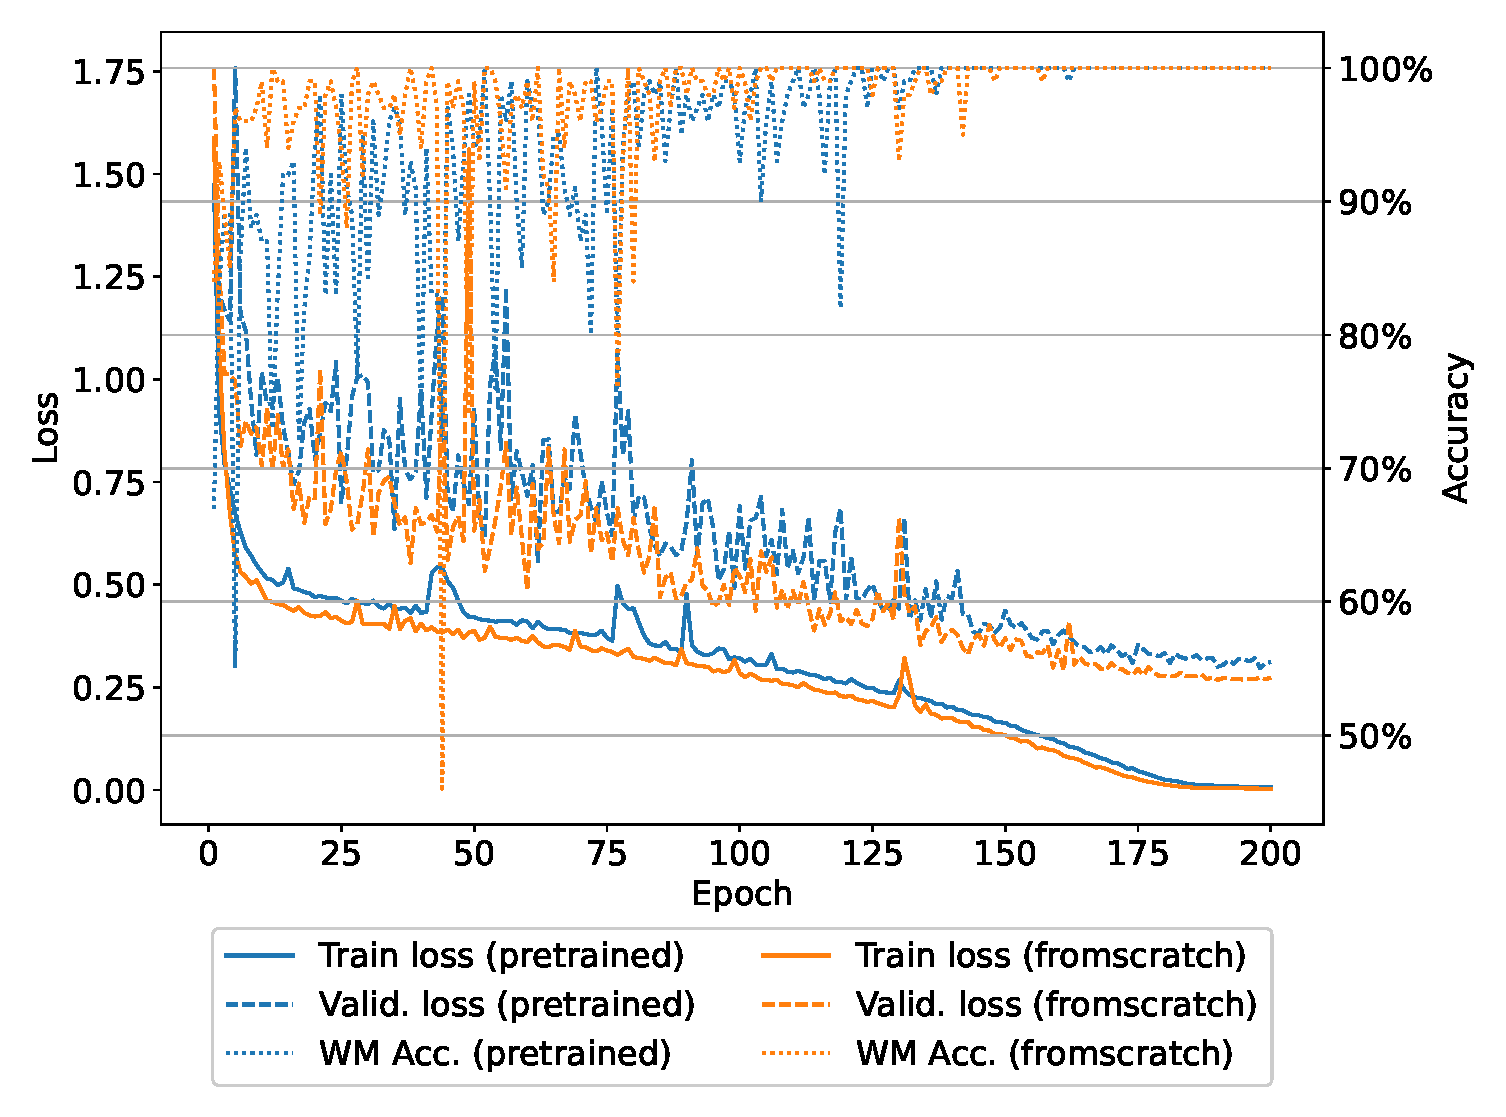
\includegraphics[width=0.7\linewidth]{images/weakness/weakness_pretrained_vs_fromscratch.eps}
    \caption{Behaviour of DenseNet during training with embedding type \textit{pretrained} and \textit{fromscratch}.}
    \label{fig:weakness-pretrained-fromscratch}
\end{figure}

We tested both embedding types on all models. For instance, \cref{fig:weakness-pretrained-fromscratch} shows the behaviour of DenseNet during watermark embedding for both embedding types. We conclude that embedding \textit{fromscratch} leads to better fidelity, which is consistent with the conclusions by the authors (cf. \cref{fig:weakness-pretrained-fromscratch}).

\subsubsection{ProtectingIP} \label{sec:compare-results:protecting}

We present the results on effectiveness from Zhang et al. \cite{zhang_protecting_2018} and our results in \cref{fig:results-effectiveness:protecting}. They tested the watermarks on a custom DNN and on MNIST and CIFAR-10.
%For "Watermarks (trained)" the model is tested on the trigger images that were in the training set and for "Watermarks (new)" the model is tested with newly generated watermarks that the model has not seen before. \textit{WM\_content} corresponds to our \textit{ProtectingIP-pattern}, \textit{WM\_unrelated} to our \textit{ProtectingIP-OOD} and \textit{WM\_noise} to our \textit{ProtectingIP-noise}.
We reach slightly better results, as our models for \textit{ProtectingIP} reach all 100\% watermark accuracy (cf. \cref{tab:effectiveness}). It is worth noting that the paper does not provide information on the trigger set size and we, therefore, cannot conclude where the difference in effectiveness could stem from.

%\begin{figure}
%    \centering
%    \includegraphics[width=0.7\linewidth]{images/protecting/protecting_effectiveness.png}
%    \caption{Results on effectiveness from Zhang et al. \cite{zhang_protecting_2018}.}
%    \label{fig:results-effectiveness:protecting}
%\end{figure}

\begin{table}
\small
\centering
\caption{Effectiveness results from Zhang et al. (\cite{zhang_protecting_2018}, Table 1), and our results.}
\label{fig:results-effectiveness:protecting}
\begin{tabular}{|l|c|c|c|c|}
\hline
                              & \multicolumn{2}{c|}{Zhang et al.'s results} & \multicolumn{2}{c|}{Our results}   \\ \hline
                              & \textbf{MNIST}  & \textbf{CIFAR-10} & \textbf{MNIST} & \textbf{CIFAR-10} \\ \hline
Method                        & WM Acc.         & WM Acc.           & WM Acc.        & WM Acc.           \\ \hline
\textit{ProtectingIP-pattern} & 100\%           & 99.93\%           & 100\%          & {\color[HTML]{036400} 100\%}             \\ \hline
\textit{ProtectingIP-OOD}     & 100\%           & 100\%             & 100\%          & 100\%             \\ \hline
\textit{ProtectingIP-noise}   & 100\%           & 99.86\%           & 100\%          & {\color[HTML]{036400} 100\%}             \\ \hline
\end{tabular}
\end{table}

Regarding robustness against pruning, we present the authors' results right beside ours in \cref{tab:results-pruning:protecting:compared}. Our results for CIFAR-10 are from ResNet-18 trained with 100 trigger images and for MNIST from LeNet-5 trained with 120 trigger images. We compare only the watermark accuracy, since we used different architectures, and mark in green and red where our models perform better resp. worse.

The most noticeable difference is that for the MNIST model watermarked with \textit{ProtectingIP-pattern} and \textit{ProtectingIP-OOD}, our watermark accuracy drops quicker. Also, for almost all models when 90\% of the parameters are pruned, the watermark accuracy of Zhang et al. is higher than ours. We again want to mention that Zhang et al. \cite{zhang_protecting_2018} used custom DNNs, which makes the results difficult to compare. Their custom DNN for MNIST has 312,202 trainable parameters, which are three times as much compared to our LeNet-5 with 107,786 trainable parameters. Their custom DNN for CIFAR-10 has 1,146,826 trainable parameters, which are only 10\% compared to our ResNet-18 with 11,173,962 trainable parameters. As they use a DNN with more parameters for MNIST, the model might have spare capacity, i.e. might be too large for the task, and thus shows such high robustness against pruning. The results for CIFAR-10 are not that clear: our models do perform better than the MNIST models but not as good as we would expect. We conclude that robustness against pruning not only depends on the complexity of the architecture but also the structure and the learned parameters itself.


%\begin{figure}
%    \centering
%    \includegraphics[width=\linewidth]{images/protecting/protecting_pruning.pdf}
%    \caption{Results on robustness against pruning from Zhang et al. \cite{zhang_protecting_2018}, Table 3 and Table 4.}
%    \label{fig:results-pruning:protecting}
%\end{figure}

% Please add the following required packages to your document preamble:
% \usepackage{multirow}
% \usepackage[table,xcdraw]{xcolor}
% If you use beamer only pass "xcolor=table" option, i.e. \documentclass[xcolor=table]{beamer}
\begin{table}
\centering
\caption{Pruning results from Zhang et al. (\cite{zhang_protecting_2018}, Table 3 and Table 4), compared with our results. "Test" stands for test accuracy, "WM" for watermark accuracy and "Pr. rate" for pruning rate.}
\label{tab:results-pruning:protecting:compared}
\resizebox{\textwidth}{!}{
\begin{tabular}{|c|cc|cc|cc|cc|cc|cc|}
\hline
\multicolumn{13}{|c|}{\textbf{MNIST}}                                                                                                                                                                                                                                                                                               \\ \hline
                           & \multicolumn{4}{c|}{\textit{ProtectingIP-pattern}}                                               & \multicolumn{4}{c|}{\textit{ProtectingIP-OOD}}                                                   & \multicolumn{4}{c|}{\textit{ProtectingIP-noise}}                                                 \\ \cline{2-13} 
                           & \multicolumn{2}{c|}{Our results}                           & \multicolumn{2}{c|}{Zhang's results} & \multicolumn{2}{c|}{Our results}                           & \multicolumn{2}{c|}{Zhang's results} & \multicolumn{2}{c|}{Our results}                           & \multicolumn{2}{c|}{Zhang's results} \\ \cline{2-13} 
\multirow{-3}{*}{Pr. rate} & \multicolumn{1}{c|}{Test} & WM                             & \multicolumn{1}{c|}{Test} & WM      & \multicolumn{1}{c|}{Test} & WM                             & \multicolumn{1}{c|}{Test} & WM      & \multicolumn{1}{c|}{Test} & WM                             & \multicolumn{1}{c|}{Test} & WM      \\ \hline
10\%                       & 98.50\%                   & 100\%                          & 99.44\%                   & 100\%   & 98.61\%                   & 100\%                          & 99.43\%                   & 100\%   & 98.48\%                   & 100\%                          & 99.4\%                    & 100\%   \\
20\%                       & 98.50\%                   & 100\%                          & 99.45\%                   & 100\%   & 98.58\%                   & 100\%                          & 99.45\%                   & 100\%   & 98.44\%                   & 100\%                          & 99.41\%                   & 100\%   \\
30\%                       & 98.30\%                   & 100\%                          & 99.43\%                   & 100\%   & 98.55\%                   & 100\%                          & 99.41\%                   & 100\%   & 98.34\%                   & 100\%                          & 99.41\%                   & 100\%   \\
40\%                       & 98.17\%                   & 100\%                          & 99.40\%                   & 100\%   & 98.45\%                   & 100\%                          & 99.31\%                   & 100\%   & 98.26\%                   & 100\%                          & 99.42\%                   & 100\%   \\
50\%                       & 98.05\%                   & 100\%                          & 99.29\%                   & 100\%   & 98.22\%                   & 100\%                          & 99.19\%                   & 100\%   & 98.21\%                   & 100\%                          & 99.41\%                   & 100\%   \\
60\%                       & 97.33\%                   & {\color[HTML]{CB0000} 98.33\%} & 99.27\%                   & 100\%   & 97.63\%                   & {\color[HTML]{CB0000} 95.83\%} & 99.24\%                   & 100\%   & 98.04\%                   & {\color[HTML]{036400} 100\%}   & 99.3\%                    & 99.9\%  \\
70\%                       & 95.84\%                   & {\color[HTML]{CB0000} 89.17\%} & 99.18\%                   & 100\%   & 96.26\%                   & {\color[HTML]{CB0000} 74.17\%} & 98.82\%                   & 100\%   & 97.96\%                   & {\color[HTML]{036400} 100\%}   & 99.22\%                   & 99.9\%  \\
80\%                       & 86.98\%                   & {\color[HTML]{CB0000} 71.67\%} & 98.92\%                   & 100\%   & 96.60\%                   & {\color[HTML]{CB0000} 75.00\%} & 97.79\%                   & 100\%   & 97.34\%                   & {\color[HTML]{036400} 100\%}   & 99.04\%                   & 99.9\%  \\
90\%                       & 71.50\%                   & {\color[HTML]{CB0000} 51.67\%} & 97.03\%                   & 99.95\% & 85.02\%                   & {\color[HTML]{CB0000} 35.00\%} & 93.55\%                   & 99.9\%  & 87.56\%                   & {\color[HTML]{CB0000} 45.83\%} & 95.19\%                   & 99.55\% \\ \hline
\multicolumn{13}{|c|}{\textbf{CIFAR-10}}                                                                                                                                                                                                                                                                                            \\ \hline
                           & \multicolumn{4}{c|}{\textit{ProtectingIP-pattern}}                                               & \multicolumn{4}{c|}{\textit{ProtectingIP-OOD}}                                                   & \multicolumn{4}{c|}{\textit{ProtectingIP-noise}}                                                 \\ \cline{2-13} 
                           & \multicolumn{2}{c|}{Our results}                           & \multicolumn{2}{c|}{Zhang's results} & \multicolumn{2}{c|}{Our results}                           & \multicolumn{2}{c|}{Zhang's results} & \multicolumn{2}{c|}{Our results}                           & \multicolumn{2}{c|}{Zhang's results} \\ \cline{2-13} 
\multirow{-3}{*}{Pr. rate} & \multicolumn{1}{c|}{Test} & WM                             & \multicolumn{1}{c|}{Test} & WM      & \multicolumn{1}{c|}{Test} & WM                             & \multicolumn{1}{c|}{Test} & WM      & \multicolumn{1}{c|}{Test} & WM                             & \multicolumn{1}{c|}{Test} & WM      \\ \hline
10\%                       & 95.02\%                   & {\color[HTML]{036400} 100\%}   & 78.37\%                   & 99.93\% & 95.28\%                   & 100\%                          & 78.06\%                   & 100\%   & 94.78\%                   & 100\%                          & 78.45\%                   & 99.86\% \\
20\%                       & 95.04\%                   & {\color[HTML]{036400} 100\%}   & 78.42\%                   & 99.93\% & 95.31\%                   & 100\%                          & 78.08\%                   & 100\%   & 94.77\%                   & 100\%                          & 78.5\%                    & 99.86\% \\
30\%                       & 95.01\%                   & {\color[HTML]{036400} 100\%}   & 78.2\%                    & 99.93\% & 95.34\%                   & 100\%                          & 78.05\%                   & 100\%   & 94.78\%                   & 100\%                          & 78.33\%                   & 99.93\% \\
40\%                       & 94.90\%                   & {\color[HTML]{036400} 100\%}   & 78.24\%                   & 99.93\% & 95.28\%                   & 100\%                          & 77.78\%                   & 100\%   & 94.84\%                   & 100\%                          & 78.31\%                   & 99.93\% \\
50\%                       & 94.75\%                   & {\color[HTML]{036400} 100\%}   & 78.16\%                   & 99.93\% & 95.25\%                   & 100\%                          & 77.75\%                   & 100\%   & 94.80\%                   & 100\%                          & 78.02\%                   & 99.8\%  \\
60\%                       & 91.91\%                   & {\color[HTML]{036400} 100\%}   & 77.87\%                   & 99.86\% & 95.01\%                   & 100\%                          & 77.44\%                   & 100\%   & 94.66\%                   & 100\%                          & 77.87\%                   & 99.6\%  \\
70\%                       & 74.76\%                   & {\color[HTML]{CB0000} 99.00\%} & 76.7\%                    & 99.86\% & 94.26\%                   & 100\%                          & 76.71\%                   & 100\%   & 94.31\%                   & 100\%                          & 77.01\%                   & 98.46\% \\
80\%                       & 54.19\%                   & {\color[HTML]{CB0000} 73.00\%} & 74.59\%                   & 99.8\%  & 88.63\%                   & {\color[HTML]{CB0000} 89.00\%} & 74.57\%                   & 96.39\% & 89.38\%                   & {\color[HTML]{036400} 94.00\%} & 73.09\%                   & 92.8\%  \\
90\%                       & 44.15\%                   & {\color[HTML]{CB0000} 31.00\%} & 64.9\%                    & 99.47\% & 15.43\%                   & {\color[HTML]{036400} 12.00\%} & 62.15\%                   & 10.93\% & 13.75\%                   & {\color[HTML]{CB0000} 13.00\%} & 59.29\%                   & 65.13\% \\ \hline
\end{tabular}
}
\end{table}

\subsubsection{FrontierStitching} \label{sec:compare-results:frontier}

Merrer et al. \cite{merrer_adversarial_2019} tested their watermarking method on two models (a CNN and an MLP, cf. \cref{tab:models-and-datasets}) on MNIST. Our results are for LeNet-1 and LeNet-3 trained with 120 trigger images. We present their and our results for robustness against pruning in \cref{fig:compare-results-pruning:frontier}. Note that the authors chose a larger step size for pruning, of 25\%, and thus not all results have a matching counterpart with our results.
In \cref{fig:compare-results-pruning:frontier}, the grey rows indicate non-plausible pruning attacks, attacks where the test accuracy fall more than 3.5\%. One may assume that their models are less complex than ours because of the quicker test and watermark accuracy drop. In fact, their both models have more trainable parameters (1,199,882 for CNN and 235,146 for MLP) compared to 69,362 for LeNet-3 and 7,206 for LeNet-1 (cf. \cref{tab:trainable_parameters}). The results for pruning are very much dependent on the model -- not only on the complexity of the architecture but the distribution of parameters in the trained model. Therefore, we cannot fully compare the results, as we used different architectures. 
%TODO: can you state what is the complexity of their models? so that we get an idea whether they are below lenet-3/-5, and whether that explains their large and quicker drop in wm accuracy? in general, one line stating that drop would be good :-)

%Comparing these results to our results for LeNet-3, which reaches 98.2\% test accuracy and 80.83\% watermark accuracy even after 90\% of the parameters were pruned, we can say that at least our LeNet-5 is more robust against pruning.

%\begin{figure}
%    \centering
%    \includegraphics[width=0.7 \linewidth]{images/frontier/frontier_pruning.pdf}
%    \caption{Results on robustness against pruning from Merrer et al. \cite{merrer_adversarial_2019}.}
%    \label{fig:results-pruning:frontier}
%\end{figure}


\begin{table}
\small
\centering
\caption{Pruning results from Merrer et al. (\cite{merrer_adversarial_2019}, Table 2), and our results. The grey cells indicate a non-plausible pruning attack. For a plausible attack and watermark accuracy above 50\% the cell is green and below it is red.}
\label{fig:compare-results-pruning:frontier}
\begin{tabular}{|c|c|c|c|c|c|c|}
\hline
\multicolumn{4}{|c|}{Merrer et al.'s results}                                                                  & \multicolumn{3}{c|}{Our results}                                          \\ \hline
Model & Pr. rate                     & Test                           & WM                            & Model   & Test                           & WM                             \\ \hline
CNN   & 20\%                         & -                              & -                             & LeNet-3 & 98.7\%                         & \cellcolor[HTML]{BAE5C5}100\%  \\ \hline
      & 25\%                         & 98.7\%                         & \cellcolor[HTML]{BAE5C5}100\% &         & -                              & -                              \\ \hline
      & 30\%                         & -                              & -                             &         & 98.7\%                         & \cellcolor[HTML]{BAE5C5}100\%  \\ \hline
      & 50\%                         & \cellcolor[HTML]{C0C0C0}88.5\% & \cellcolor[HTML]{C0C0C0}100\% &         & 98.7\%                         & \cellcolor[HTML]{BAE5C5}100\%  \\ \hline
      & 70\%                         & -                              & -                             &         & 98.7\%                         & \cellcolor[HTML]{BAE5C5}100\%  \\ \hline
      & 75\%                         & \cellcolor[HTML]{C0C0C0}42.6\% & \cellcolor[HTML]{C0C0C0}0\%   &         & -                              & -                              \\ \hline
      & 80\%                         & -                              & -                             &         & 98.7\%                         & \cellcolor[HTML]{BAE5C5}100\%  \\ \hline
      & 90\%                         & \cellcolor[HTML]{C0C0C0}25.5\% & \cellcolor[HTML]{C0C0C0}0\%   &         & 98.2\%                         & \cellcolor[HTML]{BAE5C5}80.8\% \\ \hline
MLP   & 20\%                         & -                              & -                             & LeNet-1 & 98.5\%                         & \cellcolor[HTML]{BAE5C5}100\%  \\ \hline
      & 25\%                         & 97.3\%                         & \cellcolor[HTML]{BAE5C5}100\% &         & -                              & -                              \\ \hline
      & 30\%                         & -                              & -                             &         & 98.5\%                         & \cellcolor[HTML]{BAE5C5}100\%  \\ \hline
      & 50\%                         & 96.6\%                         & \cellcolor[HTML]{BAE5C5}100\% &         & 97.6                           & \cellcolor[HTML]{BAE5C5}85\%   \\ \hline
      & 70\%                         & -                              & -                             &         & \cellcolor[HTML]{C0C0C0}87.7\% & \cellcolor[HTML]{C0C0C0}55.8\% \\ \hline
      & 75\%                         & 95.3\%                         & \cellcolor[HTML]{FFCCC9}7.7\% &         & -                              & -                              \\ \hline
      & 80\%                         & -                              & -                             &         & \cellcolor[HTML]{C0C0C0}80.7\% & \cellcolor[HTML]{C0C0C0}43.3\% \\ \hline
      & 90\%                         & \cellcolor[HTML]{C0C0C0}15.7\% & \cellcolor[HTML]{C0C0C0}0\%   &         & \cellcolor[HTML]{C0C0C0}39.8\% & \cellcolor[HTML]{C0C0C0}28.3\% \\ \hline
\end{tabular}
\end{table}

\subsubsection{WMEmbeddedSystems} \label{sec:compare-results:embedded}

Guo et al. \cite{guo_watermarking_2018} tested their watermarking method for MNIST on LeNet-5, and for CIFAR-10 on ResNet-50, DenseNet and VGG. We compare the results on fidelity for the architectures ResNet-50, DenseNet and LeNet-5. For comparison, we take the models that were trained with 100 (CIFAR-10) and 120 (MNIST) trigger images. The authors' and our results are shown in \cref{tab:results-fidelity:embedded:compared}.
%The value in parentheses in \cref{fig:results-fidelity:embedded} gives the percentage that the predicted class matches the true label.

%\begin{figure}
%    \centering
%    \includegraphics[width=0.7 \linewidth]{images/embedded/embedded_fidelity.pdf}
%    \caption{Results on fidelity from Guo et al. \cite{guo_watermarking_2018}.}
%    \label{fig:results-fidelity:embedded}
%\end{figure}

% Please add the following required packages to your document preamble:
% \usepackage{multirow}
\begin{table}
\small
\centering
\caption{Fidelity results from Guo et al. (\cite{guo_watermarking_2018}, Table 2), and our results.}
\label{tab:results-fidelity:embedded:compared}
% Please add the following required packages to your document preamble:
% \usepackage{multirow}

\begin{tabular}{ll|cccc|}
\cline{3-6}
                                                &              & \multicolumn{2}{c|}{Guo et al.'s results}                           & \multicolumn{2}{c|}{Our results}         \\ \hline
\multicolumn{1}{|l|}{Dataset}                   & Model        & \multicolumn{1}{c|}{Test Acc.} & \multicolumn{1}{c|}{WM Acc.} & \multicolumn{1}{c|}{Test Acc.} & WM Acc. \\ \hline
\multicolumn{1}{|l|}{\multirow{2}{*}{MNIST}}    & LeNet-5      & 98.99\%                        & 10\%                         & 99.23\%                        & -       \\
\multicolumn{1}{|l|}{}                          & LeNet-5 WM   & 98.48\%                        & 98.38\%                      & 99.18\%                        & {\color[HTML]{036400} 100\%}   \\ \hline
\multicolumn{1}{|l|}{\multirow{4}{*}{CIFAR-10}} & ResNet-50    & 94.53\%                        & 2.2\%                        & 94.39\%                        & -       \\
\multicolumn{1}{|l|}{}                          & ResNet-50 WM & 94.25\%                        & 99.98\%                      & {\color[HTML]{036400} 94.47\% }                       & {\color[HTML]{036400} 100\%}  \\ \cline{2-6} 
\multicolumn{1}{|l|}{}                          & DenseNet     & 94.73\%                        & 2.2\%                        & 94.58\%                        & -       \\
\multicolumn{1}{|l|}{}                          & DenseNet WM  & 94.23\%                        & 99.97\%                      & 94.10\%                        & {\color[HTML]{036400} 100\%}   \\ \hline
\end{tabular}

\end{table}

Similar to the authors, our watermarked models have a minimal test accuracy drop, below 0.5\%, and in the case of ResNet-50 even a test accuracy gain, compared to the non-watermarked models. Our models, however, reach 100\% watermark accuracy for this method, which are slightly better results than those presented by the authors.

%\subsubsection{Blackmarks} \label{sec:compare-results:blackmarks}
%\red{TODO}

\clearpage

\subsection{Effectiveness} \label{sec:eval-effectiveness}
%TODO: this should be mentioned earlier, in your study design section; you already use the term in the results earlier
%Effectiveness means that the model owner should be able to verify their watermark anytime and multiple times if needed. We show this by testing the trigger set on the watermarked model.

% Please add the following required packages to your document preamble:
% \usepackage{multirow}
% \usepackage[table,xcdraw]{xcolor}
% If you use beamer only pass "xcolor=table" option, i.e. \documentclass[xcolor=table]{beamer}
\begin{table}
\centering
\caption{Watermark accuracy on watermarked models. A checkmark \checkmark indicates 100\% watermark accuracy.}
\label{tab:effectiveness}
\setlength\tabcolsep{2pt}
\renewcommand{\arraystretch}{1.5}
\tiny 
\resizebox{\textwidth}{!}{
\begin{tabular}{|l|l|r|c|c|c|c|c|c|c|c|}
\hline
Method                                 & Type                          & Trg set size & DenseNet & ResNet-18 & ResNet-34 & ResNet-50 & SimpleNet & LeNet-1                        & LeNet-3                        & LeNet-5                        \\ \hline
                                       &                               & 20/24            & \checkmark    & \checkmark     & \checkmark     & \checkmark     & \checkmark     & \checkmark                          & \checkmark                          & \checkmark                          \\ \cline{3-11} 
                                       &                               & 100/120          & \checkmark    & \checkmark     & \checkmark     & \checkmark     & \checkmark     & \checkmark                          & \checkmark                          & \checkmark                          \\ \cline{3-11} 
                                       & \multirow{-3}{*}{pattern}     & 500/600          & \checkmark    & \checkmark     & \checkmark     & \checkmark     & \checkmark     & \checkmark                          & \checkmark                          & \checkmark                          \\ \cline{2-11} 
                                       &                               & 20/24            & \checkmark    & \checkmark     & \checkmark     & \checkmark     & \checkmark     & \checkmark                          & \checkmark                          & \checkmark                          \\ \cline{3-11} 
                                       &                               & 100/120          & \checkmark    & \checkmark     & \checkmark     & \checkmark     & \checkmark     & \checkmark                          & \checkmark                          & \checkmark                          \\ \cline{3-11} 
                                       & \multirow{-3}{*}{noise}       & 500/600          & \checkmark    & \checkmark     & \checkmark     & \checkmark     & \checkmark     & \checkmark                          & \checkmark                          & \checkmark                          \\ \cline{2-11} 
                                       &                               & 20/24            & \checkmark    & \checkmark     & \checkmark     & \checkmark     & \checkmark     & \checkmark                          & \checkmark                          & \checkmark                          \\ \cline{3-11} 
                                       &                               & 100/120          & \checkmark    & \checkmark     & \checkmark     & \checkmark     & \checkmark     & \checkmark                          & \checkmark                          & \checkmark                          \\ \cline{3-11} 
\multirow{-9}{*}{ProtectingIP}         & \multirow{-3}{*}{OOD}         & 500/600          & \checkmark    & \checkmark     & \checkmark     & \checkmark     & \checkmark     & \checkmark                          & \checkmark                          & \checkmark                          \\ \hline
                                       &                               & 20               & \checkmark    & \checkmark     & \checkmark     & \checkmark     & \checkmark     & \checkmark                          & \checkmark                          & \checkmark                          \\ \cline{3-11} 
\multirow{-2}{*}{\gape{\makecell[l]{Weakness\\IntoStrength}}} & \multirow{-2}{*}{OOD}         & 100              & \checkmark    & \checkmark     & \checkmark     & \checkmark     & \checkmark     & {\color[HTML]{CB0000} 99.00\%} & \checkmark                          & \checkmark                          \\ \hline
                                       &                               & 20/24            & \checkmark    & \checkmark     & \checkmark     & \checkmark     & \checkmark     & \checkmark                          & \checkmark                          & \checkmark                          \\ \cline{3-11} 
                                       &                               & 100/120          & \checkmark    & \checkmark     & \checkmark     & \checkmark     & \checkmark     & \checkmark                          & \checkmark                          & \checkmark                          \\ \cline{3-11} 
\multirow{-3}{*}{\gape{\makecell[l]{Piracy\\Resistant}}}      & \multirow{-3}{*}{pattern}     & 500/600          & \checkmark    & \checkmark     & \checkmark     & \checkmark     & \checkmark     & \checkmark                          & \checkmark                          & \checkmark                          \\ \hline
                                       &                               & 20/24            & \checkmark    & \checkmark     & \checkmark     & \checkmark     & \checkmark     & \checkmark                          & \checkmark                          & \checkmark                          \\ \cline{3-11} 
                                       &                               & 100/120          & \checkmark    & \checkmark     & \checkmark     & \checkmark     & \checkmark     & \checkmark                          & \checkmark                          & \checkmark                          \\ \cline{3-11} 
\multirow{-3}{*}{\gape{\makecell[l]{Exponential\\Weighting}}} & \multirow{-3}{*}{in-distrib.} & 500/600          & \checkmark    & \checkmark     & \checkmark     & \checkmark     & \checkmark     & \checkmark                          & \checkmark                          & \checkmark                          \\ \hline
                                       &                               & 20/24            & \checkmark    & \checkmark     & \checkmark     & \checkmark     & \checkmark     & \checkmark                          & \checkmark                          & \checkmark                          \\ \cline{3-11} 
                                       &                               & 100/120          & \checkmark    & \checkmark     & \checkmark     & \checkmark     & \checkmark     & \checkmark                          & \checkmark                          & {\color[HTML]{CB0000} 65.83\%} \\ \cline{3-11} 
\multirow{-3}{*}{\gape{\makecell[l]{Frontier\\Stitching}}}    & \multirow{-3}{*}{perturb.}    & 500/600          & \checkmark    & \checkmark     & \checkmark     & \checkmark     & \checkmark     & {\color[HTML]{CB0000} 65.67\%} & {\color[HTML]{CB0000} 45.33\%} & {\color[HTML]{CB0000} 45.33\%} \\ \hline
                                       &                               & 20/24            & \checkmark    & \checkmark     & \checkmark     & \checkmark     & \checkmark     & \checkmark                          & \checkmark                          & \checkmark                          \\ \cline{3-11} 
                                       &                               & 100/120          & \checkmark    & \checkmark     & \checkmark     & \checkmark     & \checkmark     & \checkmark                          & \checkmark                          & \checkmark                          \\ \cline{3-11} 
\multirow{-3}{*}{\gape{\makecell[l]{WM\\Embedded\\Systems}}}    & \multirow{-3}{*}{pattern}     & 500/600          & \checkmark    & \checkmark     & \checkmark     & \checkmark     & \checkmark     & \checkmark                          & \checkmark                          & \checkmark                          \\ \hline
\end{tabular}
}
\end{table}

From our implementations and experiments, we can confirm that almost all of the watermarking methods achieve a watermark accuracy of $100\%$. The detailed results are summarised in \cref{tab:effectiveness}. \textit{FrontierStitching} for a large trigger set size tend to lose watermark accuracy on some architectures. The models reach only around $45\%$ and $65\%$ watermark accuracy on the LeNets when trained with $600$ trigger images and also on LeNet-5 when trained with only $120$ trigger images. All of the other models have at least $99\%$ watermark accuracy, which is very much acceptable.

\clearpage

\subsection{Fidelity} \label{sec:eval-fidelity}

\Cref{fig:fidelity-perarch} shows the relative test accuracy difference as a function of the trigger set size for all watermarking methods for each architecture. From the figure, we can see that there exists a downward trend for LeNet-1, i.e. the larger the trigger set the more we lose on test accuracy.

Interestingly, all methods on SimpleNet perform exceptionally well (cf. \cref{fig:fidelity-simplenet_mnist}). We explain this by the complexity of SimpleNet and the large number of "degrees of freedom". SimpleNet is a very complex model for classifying only gray-scaled images, it consists of $51$ \textit{times} more trainable parameters than LeNet-5, the largest one of the LeNets, and almost 762 times more than LeNet-1, which shows the strongest drop in fidelity (cf. \cref{tab:trainable_parameters}).

DenseNet performs rather poorly when watermarked with \textit{ExponentialWeighting} and \textit{FrontierStitching} (cf. \cref{fig:fidelity-densenet}). This could be also explained by the (lack of) complexity of the model: DenseNet has only $30\%$ of the amount of trainable parameters compared to a ResNet-18 (cf. \cref{tab:trainable_parameters}). We can conclude that \textit{ExponentialWeighting}, an in-distribution method, fails on fidelity when used with a smaller model, as we can see it on DenseNet and LeNet-1 (cf. \cref{fig:fidelity-densenet,fig:fidelity-lenet1}).

%Also, \textit{ExponentialWeighting}, which uses in-distribution trigger images performs better on CIFAR-10 than on MNIST. Perhaps because the difference between particular images within the dataset is larger in the CIFAR-10 dataset than in the MNIST dataset and it is easier to incorrectly overfit particular images from the dataset distribution.

\begin{figure}
    \centering
    \begin{subfigure}{0.4\linewidth}
        \includegraphics[width=\linewidth]{images/fidelity/densenet_fidelity_rel_per_arch.eps}
        \caption{DenseNet trained on CIFAR-10}
        \label{fig:fidelity-densenet}
    \end{subfigure}
    \quad
    \begin{subfigure}{0.4\linewidth}
        \includegraphics[width=\linewidth]{images/fidelity/simplenet_mnist_fidelity_rel_per_arch.eps}
        \caption{SimpleNet trained on MNIST}
        \label{fig:fidelity-simplenet_mnist}
    \end{subfigure}
    \quad
    \begin{subfigure}{0.4\linewidth}
        \includegraphics[width=\linewidth]{images/fidelity/resnet18_fidelity_rel_per_arch.eps}
        \caption{ResNet-18 trained on CIFAR-10}
        \label{fig:fidelity-resnet18}
    \end{subfigure}
    \quad
    \begin{subfigure}{0.4\linewidth}
        \includegraphics[width=\linewidth]{images/fidelity/lenet1_fidelity_rel_per_arch.eps}
        \caption{LeNet-1 trained on MNIST}
        \label{fig:fidelity-lenet1}
    \end{subfigure}
    \quad
    \begin{subfigure}{0.4\linewidth}
        \includegraphics[width=\linewidth]{images/fidelity/resnet34_fidelity_rel_per_arch.eps}
        \caption{ResNet-34 trained on CIFAR-10}
        \label{fig:fidelity-resnet34}
    \end{subfigure}
    \quad
    \begin{subfigure}{0.4\linewidth}
        \includegraphics[width=\linewidth]{images/fidelity/lenet3_fidelity_rel_per_arch.eps}
        \caption{LeNet-3 trained on MNIST}
        \label{fig:fidelity-lenet3}
    \end{subfigure}
    \quad
    \begin{subfigure}{0.4\linewidth}
        \includegraphics[width=\linewidth]{images/fidelity/resnet50_fidelity_rel_per_arch.eps}
        \caption{ResNet-50 trained on CIFAR-10}
        \label{fig:fidelity-resnet50}
    \end{subfigure}
    \quad
    \begin{subfigure}{0.4\linewidth}
        \includegraphics[width=\linewidth]{images/fidelity/lenet5_fidelity_rel_per_arch.eps}
        \caption{LeNet-5 trained on MNIST}
        \label{fig:fidelity-lenet5}
    \end{subfigure}
    \quad
    
    % legend:
    \begin{subfigure}{\linewidth}
    \centering
    \includegraphics[width=0.7\linewidth]{images/fidelity/legend_fidelity_rel_per_arch.eps}
    \end{subfigure}
    
    \caption{Influence of the trigger set size on \textbf{fidelity}. Each plot corresponds to one architecture and shows the results for all watermarking methods, on the left models trained on \textbf{CIFAR-10} and on the right those trained on \textbf{MNIST}. We plot the relative difference between the test accuracy of the watermarked and non-watermarked model.}
    \label{fig:fidelity-perarch}
\end{figure}


\Cref{fig:fidelity-per-method} shows the results for fidelity but for each method. This figure confirms the conclusions from above. All methods, except of \textit{ExponentialWeighting} and \textit{FrontierStitching}, perform similarly well, i.e. the test accuracy drops for all architectures and trigger set sizes at most for around 1\% compared to the benchmark test accuracy. The worst performing models for \textit{ExponentialWeighting} are DenseNet and LeNet-1, with a big influence from the trigger set size, e.g. LeNet-1's test accuracy drops under 0.5\% when trained with only 24 trigger images, but over 4\% when trained with 600 trigger images. For \textit{FrontierStitching}, only DenseNet performs worse compared to the others with a test accuracy drop of around 2\%.

\begin{figure}
    \centering
    \begin{subfigure}{0.4\linewidth}
        \includegraphics[width=\linewidth]{images/fidelity/WeaknessIntoStrength_fidelity_rel_per_method.eps}
        \caption{WeaknessIntoStrength}
        \label{fig:fidelity-weakness}
    \end{subfigure}
    \quad
    \begin{subfigure}{0.4\linewidth}
        \includegraphics[width=\linewidth]{images/fidelity/ProtectingIP-OOD_fidelity_rel_per_method.eps}
        \caption{ProtectingIP-OOD}
        \label{fig:fidelity-ood}
    \end{subfigure}
    \quad
    \begin{subfigure}{0.4\linewidth}
        \includegraphics[width=\linewidth]{images/fidelity/ProtectingIP-pattern_fidelity_rel_per_method.eps}
        \caption{ProtectingIP-pattern}
        \label{fig:fidelity-pattern}
    \end{subfigure}
    \quad
    \begin{subfigure}{0.4\linewidth}
        \includegraphics[width=\linewidth]{images/fidelity/ProtectingIP-noise_fidelity_rel_per_method.eps}
        \caption{ProtectingIP-noise}
        \label{fig:fidelity-noise}
    \end{subfigure}
    \quad
    \begin{subfigure}{0.4\linewidth}
        \includegraphics[width=\linewidth]{images/fidelity/PiracyResistant_fidelity_rel_per_method.eps}
        \caption{PiracyResistant}
        \label{fig:fidelity-piracy}
    \end{subfigure}
    \quad
    \begin{subfigure}{0.4\linewidth}
        \includegraphics[width=\linewidth]{images/fidelity/FrontierStitching_fidelity_rel_per_method.eps}
        \caption{FrontierStitching}
        \label{fig:fidelity-frontier}
    \end{subfigure}
    \quad
    \begin{subfigure}{0.4\linewidth}
        \includegraphics[width=\linewidth]{images/fidelity/ExponentialWeighting_fidelity_rel_per_method.eps}
        \caption{ExponentialWeighting}
        \label{fig:fidelity-exponential}
    \end{subfigure}
    \quad
    \begin{subfigure}{0.4\linewidth}
        \includegraphics[width=\linewidth]{images/fidelity/WMEmbeddedSystems_fidelity_rel_per_method.eps}
        \caption{WMEmbeddedSystems}
        \label{fig:fidelity-embedded}
    \end{subfigure}
    \quad
    %\begin{subfigure}{0.4\linewidth}
    %    \includegraphics[width=\linewidth]{images/fidelity/Blackmarks_fidelity_rel_per_method.eps}
    %    \caption{Blackmarks}
    %    \label{fig:fidelity-blackmarks}
    %\end{subfigure}
    %\quad

    % legend:
    \begin{subfigure}{\linewidth}
    \centering
    \includegraphics[width=0.7\linewidth]{images/fidelity/legend_fidelity_rel_per_method.eps}
    \end{subfigure}
    
    \caption{Influence of the trigger set size on \textbf{fidelity}. Each plot corresponds to one method and shows the results for all architectures. We plot the relative difference between the test accuracy of the watermarked and non-watermarked model.}
    \label{fig:fidelity-per-method}
\end{figure}


\clearpage

\subsection{Robustness} \label{sec:eval-robustness}

\subsubsection{Parameter Pruning} \label{sec:eval-robustness-pruning}

\begin{figure}
    \centering
    \begin{subfigure}{0.4\linewidth}
        \includegraphics[width=\linewidth]{images/pruning/densenet_pruning_per_arch_08.eps}
        \caption{DenseNet, 80\% pruned.}
        \label{fig:pruning-0.8-densenet}
    \end{subfigure}
    \quad
    \begin{subfigure}{0.4\linewidth}
        \includegraphics[width=\linewidth]{images/pruning/densenet_pruning_per_arch_09.eps}
        \caption{DenseNet, 90\% pruned.}
        \label{fig:pruning-0.9-densenet}
    \end{subfigure}
    \quad
    \begin{subfigure}{0.4\linewidth}
        \includegraphics[width=\linewidth]{images/pruning/resnet18_pruning_per_arch_08.eps}
        \caption{ResNet-18, 80\% pruned.}
        \label{fig:pruning-0.8-resnet18}
    \end{subfigure}
    \quad
    \begin{subfigure}{0.4\linewidth}
        \includegraphics[width=\linewidth]{images/pruning/resnet18_pruning_per_arch_09.eps}
        \caption{ResNet-18, 90\% pruned.}
        \label{fig:pruning-0.9-resnet18}
    \end{subfigure}
    \quad
    \begin{subfigure}{0.4\linewidth}
        \includegraphics[width=\linewidth]{images/pruning/resnet34_pruning_per_arch_08.eps}
        \caption{ResNet-34, 80\% pruned.}
        \label{fig:pruning-0.8-resnet34}
    \end{subfigure}
    \quad
    \begin{subfigure}{0.4\linewidth}
        \includegraphics[width=\linewidth]{images/pruning/resnet34_pruning_per_arch_09.eps}
        \caption{ResNet-34, 90\% pruned.}
        \label{fig:pruning-0.9-resnet34}
    \end{subfigure}
    \quad
    \begin{subfigure}{0.4\linewidth}
        \includegraphics[width=\linewidth]{images/pruning/resnet50_pruning_per_arch_08.eps}
        \caption{ResNet-50, 80\% pruned.}
        \label{fig:pruning-0.8-resnet50}
    \end{subfigure}
    \quad
    \begin{subfigure}{0.4\linewidth}
        \includegraphics[width=\linewidth]{images/pruning/resnet50_pruning_per_arch_09.eps}
        \caption{ResNet-50, 90\% pruned.}
        \label{fig:pruning-0.9-resnet50}
    \end{subfigure}
    
    \begin{subfigure}{\linewidth}
    \centering
    \includegraphics[width=0.7\linewidth]{images/pruning/legend_pruning_per_arch.eps}
    \end{subfigure}
    
    \caption{Influence of the trigger set size on robustness against pruning on \textbf{CIFAR-10} models. Each plot on the left corresponds pruning with 80\% and each plot on the right to corresponds pruning with 90\%. Each plot shows the results for all watermarking methods.}
    \label{fig:pruning-cifar10models-perarch}
\end{figure}

\begin{figure}
    \centering
    \begin{subfigure}{0.4\linewidth}
        \includegraphics[width=\linewidth]{images/pruning/simplenet_mnist_pruning_per_arch_08.eps}
        \caption{SimpleNet, 80\% pruned.}
        \label{fig:pruning-0.8-simplenet}
    \end{subfigure}
    \quad
    \begin{subfigure}{0.4\linewidth}
        \includegraphics[width=\linewidth]{images/pruning/simplenet_mnist_pruning_per_arch_09.eps}
        \caption{SimpleNet, 90\% pruned.}
        \label{fig:pruning-0.9-simplenet}
    \end{subfigure}
    \quad
    \begin{subfigure}{0.4\linewidth}
        \includegraphics[width=\linewidth]{images/pruning/lenet1_pruning_per_arch_08.eps}
        \caption{LeNet-1, 80\% pruned.}
        \label{fig:pruning-0.8-lenet1}
    \end{subfigure}
    \quad
    \begin{subfigure}{0.4\linewidth}
        \includegraphics[width=\linewidth]{images/pruning/lenet1_pruning_per_arch_09.eps}
        \caption{LeNet-1, 90\% pruned.}
        \label{fig:pruning-0.9-lenet1}
    \end{subfigure}
    \quad
    \begin{subfigure}{0.4\linewidth}
        \includegraphics[width=\linewidth]{images/pruning/lenet3_pruning_per_arch_08.eps}
        \caption{LeNet-3, 80\% pruned.}
        \label{fig:pruning-0.8-lenet3}
    \end{subfigure}
    \quad
    \begin{subfigure}{0.4\linewidth}
        \includegraphics[width=\linewidth]{images/pruning/lenet3_pruning_per_arch_09.eps}
        \caption{LeNet-3, 90\% pruned.}
        \label{fig:pruning-0.9-lenet3}
    \end{subfigure}
    \quad
    \begin{subfigure}{0.4\linewidth}
        \includegraphics[width=\linewidth]{images/pruning/lenet5_pruning_per_arch_08.eps}
        \caption{LeNet-5, 80\% pruned.}
        \label{fig:pruning-0.8-lenet5}
    \end{subfigure}
    \quad
    \begin{subfigure}{0.4\linewidth}
        \includegraphics[width=\linewidth]{images/pruning/lenet5_pruning_per_arch_09.eps}
        \caption{LeNet-5, 90\% pruned.}
        \label{fig:pruning-0.9-lenet5}
    \end{subfigure}
    
    \begin{subfigure}{\linewidth}
    \centering
    \includegraphics[width=0.7\linewidth]{images/pruning/legend_pruning_per_arch.eps}
    \end{subfigure}
    
    \caption{Influence of the trigger set size on robustness against pruning on \textbf{MNIST} models. Each plot on the left corresponds pruning with 80\% and each plot on the right to corresponds pruning with 90\%. Each plot shows the results for all watermarking methods.}
    \label{fig:pruning-mnistmodels-perarch}
\end{figure}


%\begin{figure}
    \centering
    \begin{subfigure}{0.4\linewidth}
        \includegraphics[width=\linewidth]{images/pruning/densenet_pruning_per_arch_maximal_pr_rate.eps}
        \caption{DenseNet}
        \label{fig:pruning-max-pr-rate-densenet}
    \end{subfigure}
    \quad
    \begin{subfigure}{0.4\linewidth}
        \includegraphics[width=\linewidth]{images/pruning/simplenet_mnist_pruning_per_arch_maximal_pr_rate.eps}
        \caption{SimpleNet}
        \label{fig:pruning-max-pr-rate-simplenet}
    \end{subfigure}
    \quad
    \begin{subfigure}{0.4\linewidth}
        \includegraphics[width=\linewidth]{images/pruning/lenet1_pruning_per_arch_maximal_pr_rate.eps}
        \caption{ResNet-18}
        \label{fig:pruning-max-pr-rate-resnet18}
    \end{subfigure}
    \quad
    \begin{subfigure}{0.4\linewidth}
        \includegraphics[width=\linewidth]{images/pruning/lenet1_pruning_per_arch_maximal_pr_rate.eps}
        \caption{LeNet-1}
        \label{fig:pruning-max-pr-rate-lenet1}
    \end{subfigure}
    \quad
    \begin{subfigure}{0.4\linewidth}
        \includegraphics[width=\linewidth]{images/pruning/resnet34_pruning_per_arch_maximal_pr_rate.eps}
        \caption{ResNet-34}
        \label{fig:pruning-max-pr-rate-resnet34}
    \end{subfigure}
    \quad
    \begin{subfigure}{0.4\linewidth}
        \includegraphics[width=\linewidth]{images/pruning/lenet3_pruning_per_arch_maximal_pr_rate.eps}
        \caption{LeNet-3}
        \label{fig:pruning-max-pr-rate-lenet3}
    \end{subfigure}
    \quad
    \begin{subfigure}{0.4\linewidth}
        \includegraphics[width=\linewidth]{images/pruning/resnet50_pruning_per_arch_maximal_pr_rate.eps}
        \caption{ResNet-50}
        \label{fig:pruning-max-pr-rate-resnet50}
    \end{subfigure}
    \quad
    \begin{subfigure}{0.4\linewidth}
        \includegraphics[width=\linewidth]{images/pruning/lenet5_pruning_per_arch_maximal_pr_rate.eps}
        \caption{LeNet-5}
        \label{fig:pruning-max-pr-rate-lenet5}
    \end{subfigure}
    
    \begin{subfigure}{\linewidth}
    \centering
    \includegraphics[width=0.7\linewidth]{images/pruning/legend_pruning_per_arch_maximal_pr_rate.eps}
    \end{subfigure}
    
    \caption{Influence of the trigger set size on robustness against pruning with the maximal plausible pruning rate. The plots on the left correspond to models trained on \textbf{CIFAR-10} and the ones on the right to models trained on \textbf{MNIST}. Each plot shows the results for all watermarking methods.}
    \label{fig:pruning-max-pr-rate-perarch}
\end{figure}
 
%\begin{figure}
    \centering
    \begin{subfigure}{0.4\linewidth}
        \includegraphics[width=\linewidth]{images/pruning/per_method/WeaknessIntoStrength_pruning_per_method_maximal_pr_rate.eps}
        \caption{WeaknessIntoStrength}
        \label{fig:pruning-max-pr-rate-weakness}
    \end{subfigure}
    \quad
    \begin{subfigure}{0.4\linewidth}
        \includegraphics[width=\linewidth]{images/pruning/per_method/ProtectingIP-OOD_pruning_per_method_maximal_pr_rate.eps}
        \caption{ProtectingIP-OOD}
        \label{fig:pruning-max-pr-rate-ood}
    \end{subfigure}
    \quad
    \begin{subfigure}{0.4\linewidth}
        \includegraphics[width=\linewidth]{images/pruning/per_method/ProtectingIP-pattern_pruning_per_method_maximal_pr_rate.eps}
        \caption{ProtectingIP-pattern}
        \label{fig:pruning-max-pr-rate-pattern}
    \end{subfigure}
    \quad
    \begin{subfigure}{0.4\linewidth}
        \includegraphics[width=\linewidth]{images/pruning/per_method/ProtectingIP-noise_pruning_per_method_maximal_pr_rate.eps}
        \caption{ProtectingIP-noies}
        \label{fig:pruning-max-pr-rate-noise}
    \end{subfigure}
    \quad
    \begin{subfigure}{0.4\linewidth}
        \includegraphics[width=\linewidth]{images/pruning/per_method/PiracyResistant_pruning_per_method_maximal_pr_rate.eps}
        \caption{PiracyResistant}
        \label{fig:pruning-max-pr-rate-piracy}
    \end{subfigure}
    \quad
    \begin{subfigure}{0.4\linewidth}
        \includegraphics[width=\linewidth]{images/pruning/per_method/ExponentialWeighting_pruning_per_method_maximal_pr_rate.eps}
        \caption{ExponentialWeighting}
        \label{fig:pruning-max-pr-rate-exponential}
    \end{subfigure}
    \quad
    \begin{subfigure}{0.4\linewidth}
        \includegraphics[width=\linewidth]{images/pruning/per_method/FrontierStitching_pruning_per_method_maximal_pr_rate.eps}
        \caption{FrontierStitching}
        \label{fig:pruning-max-pr-rate-frontier}
    \end{subfigure}
    \quad
    \begin{subfigure}{0.4\linewidth}
        \includegraphics[width=\linewidth]{images/pruning/per_method/WMEmbeddedSystems_pruning_per_method_maximal_pr_rate.eps}
        \caption{WMEmbeddedSystems}
        \label{fig:pruning-max-pr-rate-embedded}
    \end{subfigure}
    \quad
    %\begin{subfigure}{0.4\linewidth}
    %    \includegraphics[width=\linewidth]{images/pruning/per_method/Blackmarks_pruning_per_method_maximal_pr_rate.eps}
    %    \caption{Blackmarks}
    %    \label{fig:pruning-max-pr-rate-blackmarks}
    %\end{subfigure}

    
    \begin{subfigure}{\linewidth}
    \centering
    \includegraphics[width=0.7\linewidth]{images/pruning/per_method/legend_pruning_per_method_maximal_pr_rate.eps}
    \end{subfigure}
    
    \caption{Influence of the trigger set size on robustness against pruning with the maximal plausible pruning rate. Each plot corresponds to one watermarking method and shows the results for all architectures.}
    \label{fig:pruning-max-pr-rate-permethod}
\end{figure}


The results for parameter pruning with pruning rates $80\%$ and $90\%$ for CIFAR-10 are shown in \cref{fig:pruning-cifar10models-perarch} and for MNIST in \cref{fig:pruning-mnistmodels-perarch}.

The plots show the robustness against pruning for the different sizes of trigger sets for all watermarking methods and each architecture. We clearly see that watermarks in more complex models rather resist a pruning attack with a smaller pruning rate than watermarks embedded into smaller models, as, e.g., ResNet-34 compared with ResNet-18 (cf. \cref{fig:pruning-0.8-resnet34,fig:pruning-0.8-resnet18}) or LeNet-3 compared with LeNet-1 (cf. \cref{fig:pruning-0.8-lenet3,fig:pruning-0.8-lenet1}).

Also, in some models, e.g. the LeNets, we can see a downward trend for almost all watermarking methods, i.e. a watermark with a smaller trigger set size is more robust (cf. \cref{fig:pruning-0.9-lenet1,fig:pruning-0.9-lenet3,fig:pruning-0.9-lenet5}). For CIFAR-10 models we do not see such a clear trend --  the plots across the watermarking methods do not seem to follow a pattern. Only ResNet-34 shows, for all but one watermarking method, such a trend (cf. \cref{fig:pruning-0.9-resnet34}). This observation is especially interesting, since we did not expect to see a downward trend but rather an upward trend, i.e. more trigger images lead to more robustness, as we would have expected that more trigger images in the training set would embed the watermark stronger into the model.
The downward trend could stem from the fact that most of the methods use either a random label for the trigger images, or the next label in the class vector, which means that the model does not learn to predict \textit{one specific} label for a trigger pattern, but rather has to learn combinations of features to predict the right label. For instance, for \textit{ProtectingIP-pattern} a car with the text "TEST" is labelled as "airplane", thus the model has to learn the combination of a car and the pattern in order to predict the right label. Learning such combinations might force the model parameters to adapt to a lot of small parameters instead of a few large ones. A larger trigger set size could then lead to even more of these small parameters, which then, during a pruning attack, are easily set to zero.
%The downward trend could stem from the fact that parameters responsible for the trigger images may not increase in value with the increase of trigger set size but maybe stay the same and the parameters for the original task increase in order to cope with the influence of the trigger images on the original task.
This is an assumption and could be confirmed by further experiments in future work.

%TODO: also talk about the cifar observations

%TODO: also try to explain why this downward trend exists, and what your hypothesis is/was before (i.e. did you expect this drop, or rather an increase in robustness?)

It is worth noting that the \textit{PiracyResistant} method on ResNet-34, SimpleNet and LeNet-3/5 resist even pruning with 90\% pruning rate, i.e. the watermark can still be detected with 100\% accuracy, for all trigger set sizes. This is probably related to the fact that it is the only method that uses only \textit{one} target label for the trigger images.


\begin{table}
\small
\centering
\caption{Influence of the trigger set size on robustness against pruning with the maximal plausible pruning rate. The values are the watermark accuracy after an pruning attack, the value in the parenthesis is the maximal plausible pruning rate. A checkmark \checkmark indicates 100\% watermark accuracy.}
\label{tab:max-pruning-rate}
\setlength\tabcolsep{2pt}
\renewcommand{\arraystretch}{1.5}
\tiny 
\resizebox{\textwidth}{!}{
\begin{tabular}{|l|l|r|r|r|r|r|r|r|r|r|}
\hline
Method                                 & Type                          & Trg set size & DenseNet                            & ResNet-18     & ResNet-34     & ResNet-50                           & SimpleNet     & LeNet-1                             & LeNet-3                             & LeNet-5                             \\ \hline
                                       &                               & 20/24            & 90.0\% (0.8)                        & \checkmark (0.7) & \checkmark (0.8) & \checkmark (0.8)                       & \checkmark (0.8) & 87.5\% (0.5)                        & 87.5\% (0.8)                        & 83.3\% (0.8)                        \\ \cline{3-11} 
                                       &                               & 100/120          & \checkmark (0.8)                       & \checkmark (0.6) & \checkmark (0.8) & \checkmark (0.8)                       & \checkmark (0.7) & 69.2\% (0.5)                        & 95.0\% (0.7)                        & 89.2\% (0.7)                        \\ \cline{3-11} 
                                       & \multirow{-3}{*}{pattern}     & 500/600          & 99.0\% (0.8)                        & \checkmark (0.6) & 92.0\% (0.8)  & \checkmark (0.8)                       & \checkmark (0.7) & 95.3\% (0.2)                        & 76.8\% (0.7)                        & 90.0\% (0.6)                        \\ \cline{2-11} 
                                       &                               & 20/24            & 95.0\% (0.8)                        & \checkmark (0.7) & \checkmark (0.8) & \checkmark (0.8)                       & \checkmark (0.7) & \checkmark (0.6)                       & \checkmark (0.8)                       & \checkmark (0.8)                       \\ \cline{3-11} 
                                       &                               & 100/120          & 98.0\% (0.8)                        & \checkmark (0.7) & \checkmark (0.8) & \checkmark (0.8)                       & \checkmark (0.8) & 63.3\% (0.7)                        & 98.3\% (0.8)                        & 91.7\% (0.7)                        \\ \cline{3-11} 
                                       & \multirow{-3}{*}{noise}       & 500/600          & 96.8\% (0.8)                        & \checkmark (0.5) & \checkmark (0.8) & \checkmark (0.8)                       & \checkmark (0.8) & 53.5\% (0.6)                        & 72.3\% (0.7)                        & 84.0\% (0.7)                        \\ \cline{2-11} 
                                       &                               & 20/24            & \checkmark (0.8)                       & \checkmark (0.8) & \checkmark (0.8) & \checkmark (0.8)                       & \checkmark (0.8) & 79.2\% (0.5)                        & 95.8\% (0.8)                        & 91.7\% (0.8)                        \\ \cline{3-11} 
                                       &                               & 100/120          & \checkmark (0.8)                       & \checkmark (0.7) & \checkmark (0.8) & 99.0\% (0.9)                        & \checkmark (0.8) & 86.7\% (0.5)                        & 90.0\% (0.7)                        & 75.0\% (0.8)                        \\ \cline{3-11} 
\multirow{-9}{*}{ProtectingIP}         & \multirow{-3}{*}{OOD}         & 500/600          & {\color[HTML]{CB0000} 17.6\% (0.8)} & \checkmark (0.6) & \checkmark (0.8) & 98.8\% (0.8)                        & \checkmark (0.7) & {\color[HTML]{CB0000} 41.7\% (0.5)} & 88.7\% (0.7)                        & 70.8\% (0.7)                        \\ \hline
                                       &                               & 20               & \checkmark (0.8)                       & \checkmark (0.7) & \checkmark (0.8) & \checkmark (0.8)                       & \checkmark (0.8) & {\color[HTML]{CB0000} 45.0\% (0.6)} & 65.0\% (0.9)                        & 85.0\% (0.9)                        \\ \cline{3-11} 
\multirow{-2}{*}{\gape{\makecell[l]{Weakness\\IntoStrength}}} & \multirow{-2}{*}{OOD}         & 100              & \checkmark (0.8)                       & \checkmark (0.7) & \checkmark (0.8) & {\color[HTML]{036400} \checkmark (0.9)}                       & \checkmark (0.8) & 56.0\% (0.5)                        & 73.0\% (0.9)                        & 57.0\% (0.9)                        \\ \hline
                                       &                               & 20/24            & \checkmark (0.8)                       & 75.0\% (0.8)  & {\color[HTML]{036400} \checkmark (0.9)} & {\color[HTML]{CB0000} 25.0\% (0.9)} & \checkmark (0.7) & \checkmark (0.5)                       & \checkmark (0.8)                       & \checkmark (0.7)                       \\ \cline{3-11} 
                                       &                               & 100/120          & \checkmark (0.8)                       & \checkmark (0.7) & \checkmark (0.8) & 98.0\% (0.9)                        & \checkmark (0.7) & \checkmark (0.6)                       & 99.2\% (0.9)                        & \checkmark (0.7)                       \\ \cline{3-11} 
\multirow{-3}{*}{\gape{\makecell[l]{Piracy\\Resistant}}}      & \multirow{-3}{*}{pattern}     & 500/600          & \checkmark (0.8)                       & \checkmark (0.8) & \checkmark (0.8) & 85.2\% (0.9)                        & \checkmark (0.7) & \checkmark (0.4)                       & \checkmark (0.8)                       & \checkmark (0.6)                       \\ \hline
                                       &                               & 20/24            & {\color[HTML]{036400} \checkmark (0.9)}                       & \checkmark (0.8) & {\color[HTML]{036400} \checkmark (0.9)} & {\color[HTML]{036400} \checkmark (0.9)}                       & \checkmark (0.8) & 87.5\% (0.5)                        & {\color[HTML]{036400} \checkmark (0.9)}                       & {\color[HTML]{036400} \checkmark (0.9)}                       \\ \cline{3-11} 
                                       &                               & 100/120          & {\color[HTML]{036400} \checkmark (0.9)}                       & \checkmark (0.8) & {\color[HTML]{036400} \checkmark (0.9)} & {\color[HTML]{036400} \checkmark (0.9)}                       & \checkmark (0.8) & 94.2\% (0.4)                        & 95.8\% (0.9)                        & 95.0\% (0.9)                        \\ \cline{3-11} 
\multirow{-3}{*}{\gape{\makecell[l]{Exponential\\Weighting}}} & \multirow{-3}{*}{in-distrib.} & 500/600          & -                                   & \checkmark (0.8) & 94.4\% (0.9)  & {\color[HTML]{036400} \checkmark (0.9)}                       & \checkmark (0.8) & -                                   & 83.0\% (0.9)                        & \checkmark (0.8)                       \\ \hline
                                       &                               & 20/24            & {\color[HTML]{036400} \checkmark (0.9)}                       & \checkmark (0.8) & {\color[HTML]{036400} \checkmark (0.9)} & {\color[HTML]{036400} \checkmark (0.9)}                       & \checkmark (0.8) & 87.5\% (0.6)                        & {\color[HTML]{036400} \checkmark (0.9)}                       & 91.7\% (0.9)                        \\ \cline{3-11} 
                                       &                               & 100/120          & {\color[HTML]{036400} \checkmark (0.9)}                       & \checkmark (0.8) & {\color[HTML]{036400} \checkmark (0.9)} & {\color[HTML]{036400} \checkmark (0.9)}                       & \checkmark (0.8) & 85.0\% (0.5)                        & 80.8\% (0.9)                        & {\color[HTML]{CB0000} 45.8\% (0.9)} \\ \cline{3-11} 
\multirow{-3}{*}{\gape{\makecell[l]{Frontier\\Stitching}}}    & \multirow{-3}{*}{perturb.}    & 500/600          & 98.6\% (0.9)                        & \checkmark (0.8) & 79.2\% (0.9)  & 96.4\% (0.9)                        & \checkmark (0.8) & {\color[HTML]{CB0000} 42.5\% (0.6)} & {\color[HTML]{CB0000} 30.3\% (0.9)} & {\color[HTML]{CB0000} 25.3\% (0.9)} \\ \hline
                                       &                               & 20/24            & \checkmark (0.8)                       & \checkmark (0.7) & \checkmark (0.8) & 95.0\% (0.9)                        & \checkmark (0.8) & 79.2\% (0.7)                        & {\color[HTML]{036400} \checkmark (0.9)}                       & {\color[HTML]{036400} \checkmark (0.9)}                       \\ \cline{3-11} 
                                       &                               & 100/120          & \checkmark (0.8)                       & \checkmark (0.6) & \checkmark (0.8) & \checkmark (0.8)                       & 97.5\% (0.8)  & 83.3\% (0.7)                        & 61.7\% (0.9)                        & 96.7\% (0.9)                        \\ \cline{3-11} 
\multirow{-3}{*}{\gape{\makecell[l]{WMEmbedded\\Systems}}}    & \multirow{-3}{*}{pattern}     & 500/600          & 98.0\% (0.8)                        & \checkmark (0.6) & \checkmark (0.7) & \checkmark (0.8)                       & \checkmark (0.6) & 82.17\% (0.5)                       & 82.5\% (0.8)                        & 94.2\% (0.8)                        \\ \hline
\end{tabular}
}
\end{table}

%Meisten 100\% --> SimpleNet und ResNet-18, aber SimpleNet trotzdem besser.
%Wenigsten 100\% --> LeNet-1

Since we do not assume that an attacker would perform a pruning attack regardless of how much the model loses in test accuracy (as the 'value' of the model would then also decrease), we test the watermark accuracy of a model at the maximal plausible pruning rate, as discussed in \cref{sec:implementation:pruning}, and show the results in \cref{tab:max-pruning-rate}. The values below 50\% watermark accuracy are marked in red, and we consider these models as not robust against pruning. However, it depends on the watermark accuracy threshold the model owner sets. Those models without a value in the table are models that performed already badly on fidelity, i.e. having more than 3.5\% test accuracy drop. Models reaching a 100\% watermark accuracy after 90\% of the weights are pruned are marked green.

From this table, we conclude that a watermark in a smaller model like LeNet-1 is less robust against pruning than in a more complex model like SimpleNet or ResNet-18. Note that we performed pruning with a step size of 10 percentage points and these results could change when tested with, e.g., a step size of 1 percentage point. We see that those models that fail on pruning are trained with an OOD or perturbation based method, and also ResNet-50 with PiracyResistant and trigger set size 20. However, those perturbation based models that seem to perform badly in this table are also those models that reach only 45-65 \% watermark accuracy after the embedding.
Therefore, instead of declaring them as not robust against pruning, we rather declare them as primarily not effective.

We can see that the watermarking methods most robust against pruning are \textit{ProtectingIP-pattern}, \textit{ProtectingIP-noise} and \textit{ExponentialWeighting}. For those, the watermark accuracy, after a pruning attack with the maximal plausible pruning rate, stays above 50\% for all architectures and all trigger set sizes. For \textit{ExponentialWeighting}, even the worst-performing model has a watermark accuracy of 83\%, but two models, DenseNet with the trigger set size 500 and LeNet-1 with the trigger set size 600, did not even qualify for pruning since they already fail the fidelity requirement.

\clearpage

\subsubsection{Fine-Tuning} \label{sec:eval-robustness-finetuning}

\begin{figure}
    \centering
    \begin{subfigure}{0.41\linewidth}
        \includegraphics[width=\linewidth]{images/finetuning/densenet_finetuning_per_arch_00001.eps}
        \caption{DenseNet, fine-tuned with $\alpha=10^{-4}$}
        \label{fig:finetuning-smalllr-allmethods-perarch-densenet}
    \end{subfigure}
    \quad
    \begin{subfigure}{0.41\linewidth}
        \includegraphics[width=\linewidth]{images/finetuning/densenet_finetuning_per_arch_001.eps}
        \caption{DenseNet, fine-tuned with $\alpha=10^{-2}$}
        \label{fig:finetuning-largelr-allmethods-perarch-densenet}
    \end{subfigure}
    \quad
    \begin{subfigure}{0.41\linewidth}
        \includegraphics[width=\linewidth]{images/finetuning/resnet18_finetuning_per_arch_00001.eps}
        \caption{ResNet-18, fine-tuned with $\alpha=10^{-4}$}
        \label{fig:finetuning-smalllr-allmethods-perarch-resnet18}
    \end{subfigure}
    \quad
    \begin{subfigure}{0.41\linewidth}
        \includegraphics[width=\linewidth]{images/finetuning/resnet18_finetuning_per_arch_001.eps}
        \caption{ResNet-18, fine-tuned with $\alpha=10^{-2}$}
        \label{fig:finetuning-largelr-allmethods-perarch-resnet18}
    \end{subfigure}
    \quad
    \begin{subfigure}{0.41\linewidth}
        \includegraphics[width=\linewidth]{images/finetuning/resnet34_finetuning_per_arch_00001.eps}
        \caption{ResNet-34, fine-tuned with $\alpha=10^{-4}$}
        \label{fig:finetuning-smalllr-allmethods-perarch-resnet34}
    \end{subfigure}
    \quad
    \begin{subfigure}{0.41\linewidth}
        \includegraphics[width=\linewidth]{images/finetuning/resnet34_finetuning_per_arch_001.eps}
        \caption{ResNet-34, fine-tuned with $\alpha=10^{-2}$}
        \label{fig:finetuning-largelr-allmethods-perarch-resnet34}
    \end{subfigure}
    \quad
    \begin{subfigure}{0.41\linewidth}
        \includegraphics[width=\linewidth]{images/finetuning/resnet50_finetuning_per_arch_00001.eps}
        \caption{ResNet-50, fine-tuned with $\alpha=10^{-4}$}
        \label{fig:finetuning-smalllr-allmethods-perarch-resnet50}
    \end{subfigure}
    \quad
    \begin{subfigure}{0.41\linewidth}
        \includegraphics[width=\linewidth]{images/finetuning/resnet50_finetuning_per_arch_001.eps}
        \caption{ResNet-50, fine-tuned with $\alpha=10^{-2}$}
        \label{fig:finetuning-largelr-allmethods-perarch-resnet50}
    \end{subfigure}
    
    \begin{subfigure}{\linewidth}
    \centering
    \includegraphics[height=1cm]{images/finetuning/legend_finetuning_per_arch_colors.eps}
    %\quad
    %\includegraphics[height=1cm]{images/finetuning/legend_finetuning_per_arch_linestyles.eps}
    \end{subfigure}
    
    \caption{Influence of the trigger set size on robustness against fine-tuning on \textbf{CIFAR-10} models. Each plot on the right corresponds fine-tuning with a small learning rate and each plot on the left to fine-tuning with a large learning rate, all of them show the results for all watermarking methods.}
    \label{fig:finetuning-cifar10models-perarch}
\end{figure}
% The black dash-dotted line corresponds to the benchmark test accuracy of the non-watermarked model.

\begin{figure}
    \centering
    \begin{subfigure}{0.41\linewidth}
        \includegraphics[width=\linewidth]{images/finetuning/simplenet_mnist_finetuning_per_arch_1e-05.eps}
        \caption{SimpleNet, fine-tuned with $\alpha=10^{-5}$}
        \label{fig:finetuning-smalllr-allmethods-perarch-simplenet_mnist}
    \end{subfigure}
    \quad
    \begin{subfigure}{0.41\linewidth}
        \includegraphics[width=\linewidth]{images/finetuning/simplenet_mnist_finetuning_per_arch_001.eps}
        \caption{SimpleNet, fine-tuned with $\alpha=10^{-2}$}
        \label{fig:finetuning-largelr-allmethods-perarch-simplenet_mnist}
    \end{subfigure}
    \quad
    \begin{subfigure}{0.41\linewidth}
        \includegraphics[width=\linewidth]{images/finetuning/lenet1_finetuning_per_arch_1e-05.eps}
        \caption{LeNet-1, fine-tuned with $\alpha=10^{-5}$}
        \label{fig:finetuning-smalllr-allmethods-perarch-lenet1}
    \end{subfigure}
    \quad
    \begin{subfigure}{0.41\linewidth}
        \includegraphics[width=\linewidth]{images/finetuning/lenet1_finetuning_per_arch_001.eps}
        \caption{LeNet-1, fine-tuned with $\alpha=10^{-2}$}
        \label{fig:finetuning-largelr-allmethods-perarch-lenet1}
    \end{subfigure}
    \quad
    \begin{subfigure}{0.41\linewidth}
        \includegraphics[width=\linewidth]{images/finetuning/lenet3_finetuning_per_arch_1e-05.eps}
        \caption{LeNet-3, fine-tuned with $\alpha=10^{-5}$}
        \label{fig:finetuning-smalllr-allmethods-perarch-lenet3}
    \end{subfigure}
    \quad
    \begin{subfigure}{0.41\linewidth}
        \includegraphics[width=\linewidth]{images/finetuning/lenet3_finetuning_per_arch_001.eps}
        \caption{LeNet-3, fine-tuned with $\alpha=10^{-2}$}
        \label{fig:finetuning-largelr-allmethods-perarch-lenet3}
    \end{subfigure}
    \quad
    \begin{subfigure}{0.41\linewidth}
        \includegraphics[width=\linewidth]{images/finetuning/lenet5_finetuning_per_arch_1e-05.eps}
        \caption{LeNet-5, fine-tuned with $\alpha=10^{-5}$}
        \label{fig:finetuning-smalllr-allmethods-perarch-lenet5}
    \end{subfigure}
    \quad
    \begin{subfigure}{0.41\linewidth}
        \includegraphics[width=\linewidth]{images/finetuning/lenet5_finetuning_per_arch_001.eps}
        \caption{LeNet-5, fine-tuned with $\alpha=10^{-2}$}
        \label{fig:finetuning-largelr-allmethods-perarch-lenet5}
    \end{subfigure}
    
    \begin{subfigure}{\linewidth}
    \centering
    \includegraphics[height=1cm]{images/finetuning/legend_finetuning_per_arch_colors.eps}
    %\quad
    %\includegraphics[height=1cm]{images/finetuning/legend_finetuning_per_arch_linestyles.eps}
    \end{subfigure}
    
    \caption{Influence of the trigger set size on robustness against fine-tuning on MNIST models. Each plot on the left corresponds fine-tuning with a small learning rate and each plot on the right to fine-tuning with a large learning rate, all of them show the results for all watermarking methods.}
    \label{fig:finetuning-mnistmodels-perarch}
\end{figure}
% The black dash-dotted line corresponds to the benchmark test accuracy of the non-watermarked model.

The results for fine-tuning for CIFAR-10 are shown in \cref{fig:finetuning-cifar10models-perarch} and for MNIST in \cref{fig:finetuning-mnistmodels-perarch}.

For fine-tuning with a smaller learning rate, we can see a downward trend for most of the watermarking methods trained on models classifying CIFAR-10 (cf. \cref{fig:finetuning-cifar10models-perarch}). For MNIST models we cannot detect such a trend, neither downward nor upward (cf. \cref{fig:finetuning-mnistmodels-perarch}). For fine-tuning with a larger learning rate, all watermarking methods on all architectures for all trigger set sizes fail to resist, the watermark accuracies are mostly below $20\%$. Again, as discussed above, we did not expect a downward trend regarding robustness but rather an upward trend, i.e. more trigger images lead to more robustness. We discuss this observation in more detail after we analysed the fine-tuning plots per method.
%TODO explain why this could happen...

\begin{figure}
    \centering
    \begin{subfigure}[b]{\linewidth}
    \centering
    \includegraphics[width=0.7 \linewidth]{images/finetuning/finetuning_protecting_content_trgsetsizes_thesis_resnet18.eps}
    \end{subfigure}
    \begin{subfigure}[b]{\linewidth}
    \centering
    \includegraphics[height=1cm]{images/finetuning/legend_finetuning_protecting_content_trgsetsizes_colors.eps}
    \quad
    \includegraphics[height=1cm]{images/finetuning/legend_finetuning_protecting_content_trgsetsizes_linetypes.eps}
    \end{subfigure}
    \caption{Behaviour of ResNet-18 watermarked with \textit{ProtectingIP-pattern} during a fine-tuning attack with a small learning rate $\alpha=10^{-4}$. The colors indicate the trigger set size, with which the model was watermarked. The black dash-dotted line corresponds to the benchmark test accuracy of the non-watermarked model.}
    \label{fig:finetuning-content-trgsetsizes}
\end{figure}

Also, \cref{fig:finetuning-content-trgsetsizes} shows that, during a fine-tuning attack, the model trained with a larger trigger set size (500) loses watermark accuracy more quickly.

Also here, we can see that SimpleNet performs best for both fine-tuning settings (cf. \cref{fig:finetuning-smalllr-allmethods-perarch-simplenet_mnist,fig:finetuning-largelr-allmethods-perarch-simplenet_mnist}). Overall, the highest watermark accuracies are seen on SimpleNet. Interestingly, for SimpleNet a \textit{larger} trigger set size is beneficial, since models with smaller trigger set sizes lose more watermark accuracy after fine-tuning with a smaller learning rate.

\begin{figure}
    \centering
    \begin{subfigure}{0.41\linewidth}
        \includegraphics[width=\linewidth]{images/finetuning/WeaknessIntoStrength_finetuning_per_method_smalllr.eps}
        \caption{WeaknessIntoStrength}
        \label{fig:finetuning-smalllr-permethod-weakness}
    \end{subfigure}
    \quad
    \begin{subfigure}{0.41\linewidth}
        \includegraphics[width=\linewidth]{images/finetuning/ProtectingIP-OOD_finetuning_per_method_smalllr.eps}
        \caption{ProtectingIP-OOD}
        \label{fig:finetuning-smalllr-permethod-ood}
    \end{subfigure}
    \quad
    \begin{subfigure}{0.41\linewidth}
        \includegraphics[width=\linewidth]{images/finetuning/ProtectingIP-pattern_finetuning_per_method_smalllr.eps}
        \caption{ProtectingIP-pattern}
        \label{fig:finetuning-smalllr-permethod-pattern}
    \end{subfigure}
    \quad
    \begin{subfigure}{0.41\linewidth}
        \includegraphics[width=\linewidth]{images/finetuning/ProtectingIP-noise_finetuning_per_method_smalllr.eps}
        \caption{ProtectingIP-noies}
        \label{fig:finetuning-smalllr-permethod-noise}
    \end{subfigure}
    \quad
    \begin{subfigure}{0.41\linewidth}
        \includegraphics[width=\linewidth]{images/finetuning/PiracyResistant_finetuning_per_method_smalllr.eps}
        \caption{PiracyResistant}
        \label{fig:finetuning-smalllr-permethod-piracy}
    \end{subfigure}
    \quad
    \begin{subfigure}{0.41\linewidth}
        \includegraphics[width=\linewidth]{images/finetuning/ExponentialWeighting_finetuning_per_method_smalllr.eps}
        \caption{ExponentialWeighting}
        \label{fig:finetuning-smalllr-permethod-exponential}
    \end{subfigure}
    \quad
    \begin{subfigure}{0.41\linewidth}
        \includegraphics[width=\linewidth]{images/finetuning/FrontierStitching_finetuning_per_method_smalllr.eps}
        \caption{FrontierStitching}
        \label{fig:finetuning-smalllr-permethod-frontier}
    \end{subfigure}
    \quad
    \begin{subfigure}{0.41\linewidth}
        \includegraphics[width=\linewidth]{images/finetuning/WMEmbeddedSystems_finetuning_per_method_smalllr.eps}
        \caption{WMEmbeddedSystems}
        \label{fig:finetuning-smalllr-permethod-embedded}
    \end{subfigure}
    \quad
    %\begin{subfigure}{0.41\linewidth}
    %    \includegraphics[width=\linewidth]{images/finetuning/Blackmarks_finetuning_per_method_smalllr.eps}
    %    \caption{Blackmarks}
    %    \label{fig:finetuning-smalllr-permethod-blackmarks}
    %\end{subfigure}

    
    \begin{subfigure}{\linewidth}
    \centering
    \includegraphics[width=0.7\linewidth]{images/finetuning/legend_finetuning_per_method_colors.eps}
    \end{subfigure}
    
    \caption{Influence of the trigger set size on robustness against fine-tuning with a small learning rate, $10^{-5}$ for MNIST and  $10^{-4}$ for CIFAR-10. Each plot corresponds to one watermarking method and shows the results for all architectures.}
    \label{fig:finetuning-smalllr-permethod}
\end{figure}


Concluding this section, \cref{fig:finetuning-smalllr-permethod} shows the results for fine-tuning with a smaller learning rate ($\alpha=10^{-4}$ for CIFAR-10 and $\alpha=10^{-5}$ for MNIST) for all architectures for each watermarking method. Comparing each watermarking method, we can see an upward trend in \textit{WeaknessIntoStrength} (cf. \cref{fig:finetuning-smalllr-permethod-weakness}) for almost all architectures, but we do see this also for other methods comparing trigger set size 20 and 100. A downward trend can be detected for \textit{ExponentialWeighting}, \textit{FrontierStitching}, \textit{ProtectingIP-pattern} and \textit{ProtectingIP-OOD} (cf. \cref{fig:finetuning-smalllr-permethod-exponential,fig:finetuning-smalllr-permethod-frontier,fig:finetuning-smalllr-permethod-pattern,fig:finetuning-smalllr-permethod-ood}). The reason for the downward trend might be the same as for pruning. These methods do use more than one label for the trigger images and therefore the model does not learn the specific trigger "pattern", but overfits on every single trigger image, which the model then easily "forgets" during a fine-tuning attack.

Note that \textit{WeaknessIntoStrength} was trained only with 20 and 100 trigger images and therefore we do not have the same amount of information compared to the other ones. Although \textit{ExponentialWeighting} shows a downward trend, the watermark accuracy for the models trained with 100/120 trigger images are among the highest compared to other methods. We observe the same for \textit{WMEmbeddedSystems}, as the watermark accuracy for those trigger set sizes is above 60\%.

Interestingly, MNIST models watermarked with \textit{PiracyResistant} have a watermark accuracy of 100\% even after a fine-tuning attack with a small learning rate. This, however, is not the case for CIFAR-10 models, as the watermark accuracy for those models is between 20\% and 40\% after the fine-tuning attack. As above, this high robustness of MNIST models might be related to the fact that \textit{PiracyResistant} uses one label for all trigger images. 



%Recall that for fidelity, \textit{ExponentialWeighting} also showed an downward trend for smaller models, such as DenseNet and LeNet-1 (cf. \cref{sec:eval-fidelity}).

% KEINE EMPFEHLUNG FÜR EXPONENTIALWEIGHTING AUF KLEINEREN MODELLEN UND GRÖSSERE TRG SET SIZES- sowohl für fidelity als auch robustness fine-tuning

% Upward trend: Weakness
% Downward trend Exponential, Protecting IP prattern, FrontierStitching

% Haben auch schon bei fildeity gesehen, dass exponential und weakness mit gr trigger set size nicht so gut klarkommen...

%paper \textbf{Deep Signs Fine-tuning:}
%"We use the same learning rate as the one in the final stage of DL training to perform model fine-tuning attack. As shown in Table 3, DeepSigns can successfully detect the embedded WM even after fine-tuning the DNN for various number of epochs. We set the number of fine-tuning epochs to 10 and 20 epochs for ImageNet benchmark and 50, 100, 200 epochs for other benchmarks. The reason for this selection is that training the ImageNet benchmark from scratch takes 90 epochs whereas other benchmarks take around 300 epochs to be trained."

%paper \textbf{How To Prove:}
%"For example, an attacker can fine-tune the stolen model to achieve the purpose of removing the watermark. More often in practice, it is common to fine-tune the existing state-of-the-art models on new insufficient datasets to achieve higher performance or to implement new tasks. trains another 100 epochs."

%Training a high-performance model from scratch requires a lot of resources, and insufficient datasets can significantly affect the performance of the model. Fine-tuning is a common strategy in practice, and we can fine-tune pre-trained models to complete new tasks or achieve higher performance. Therefore, an attacker can fine-tune the stolen model with fewer new datasets to obtain a new model that inherits the performance of the stolen model but is also different from the stolen model.

%In this experiment, we divide the test set into two halves. The first half (80\%) is used for fine-tuning pre-trained models while the second half (20\%) is used for evaluating new models. We use watermark (key samples) accuracy of new models to measure the ro- bustness of our framework for modifications caused by fine-tuning.

%paper \textbf{WMEmbeddedSystems}:
%We assume that attackers are those who want to use a “pirate model” without paying the royalty. The attackers do not have the computa- tion power and technical expertise to train a model of their own. Uchida et al. argue that transfer learning and model compression operations, in particular, should be considered as possible types of attacks [6]. We do not consider them a type of threat for the follow- ing reasons. First, the cost of fine-tuning and compression is on the same order of magnitude as the cost of training, if not higher [13]. With that much resources and expertise at hand, an attacker would have built a model on their own. Second, a fine-tuned model is essentially a different model with certain initialization. In our own experiment for fine-tuning between different datasets, we observe up to 93\% difference in average magnitude of weights in a layer. Not to mention that model architecture may be changed during the pruning of a model [14][2]. We argue the proof-of-authorship during actual model usage and “proof-of-origin” of a model should be two different problems. It is questionable whether the original model author can claim the authorship of a fine-tuned model, and thus our assumption.

%paper \textbf{Uchida: Embedding Watermarks}
%The Caltech-101 dataset [10] includes pictures of objects belonging to 101 categories; it contains about 40 to 800 images per category. The size of each image is roughly 300 × 200 pixels but we resized them in 32 × 32 for fine-tuning. For each category, we used 30 images for training and at most 40 of the remaining images for testing.

%Fine-tuningortransferlearn- ing [28] seems to be the most likely type of (unintentional) attack because it is frequently performed on trained models to apply them to other but similar tasks with less effort than training a network from scratch or to avoid over-fitting when sufficient training data is not available.

%Did same domain CIFAR-10 -> CIFAR-10 and other domain Caltech-101 -> CIFAR-10.